\documentclass[10pt,a4paper]{article}
\usepackage{lmodern}
\usepackage{amssymb,amsmath}
\usepackage{ifxetex,ifluatex}
\usepackage{fixltx2e} % provides \textsubscript
\ifnum 0\ifxetex 1\fi\ifluatex 1\fi=0 % if pdftex
  \usepackage[T1]{fontenc}
  \usepackage[utf8]{inputenc}
\else % if luatex or xelatex
  \ifxetex
    \usepackage{mathspec}
    \usepackage{xltxtra,xunicode}
  \else
    \usepackage{fontspec}
  \fi
  \defaultfontfeatures{Mapping=tex-text,Scale=MatchLowercase}
  \newcommand{\euro}{€}
\fi
% use upquote if available, for straight quotes in verbatim environments
\IfFileExists{upquote.sty}{\usepackage{upquote}}{}
% use microtype if available
\IfFileExists{microtype.sty}{%
\usepackage{microtype}
\UseMicrotypeSet[protrusion]{basicmath} % disable protrusion for tt fonts
}{}
\usepackage{color}
\usepackage{fancyvrb}
\newcommand{\VerbBar}{|}
\newcommand{\VERB}{\Verb[commandchars=\\\{\}]}
\DefineVerbatimEnvironment{Highlighting}{Verbatim}{commandchars=\\\{\}}
% Add ',fontsize=\small' for more characters per line
\usepackage{framed}
\definecolor{shadecolor}{RGB}{248,248,248}
\newenvironment{Shaded}{\begin{snugshade}}{\end{snugshade}}
\newcommand{\AlertTok}[1]{\textcolor[rgb]{0.94,0.16,0.16}{#1}}
\newcommand{\AnnotationTok}[1]{\textcolor[rgb]{0.56,0.35,0.01}{\textbf{\textit{#1}}}}
\newcommand{\AttributeTok}[1]{\textcolor[rgb]{0.77,0.63,0.00}{#1}}
\newcommand{\BaseNTok}[1]{\textcolor[rgb]{0.00,0.00,0.81}{#1}}
\newcommand{\BuiltInTok}[1]{#1}
\newcommand{\CharTok}[1]{\textcolor[rgb]{0.31,0.60,0.02}{#1}}
\newcommand{\CommentTok}[1]{\textcolor[rgb]{0.56,0.35,0.01}{\textit{#1}}}
\newcommand{\CommentVarTok}[1]{\textcolor[rgb]{0.56,0.35,0.01}{\textbf{\textit{#1}}}}
\newcommand{\ConstantTok}[1]{\textcolor[rgb]{0.00,0.00,0.00}{#1}}
\newcommand{\ControlFlowTok}[1]{\textcolor[rgb]{0.13,0.29,0.53}{\textbf{#1}}}
\newcommand{\DataTypeTok}[1]{\textcolor[rgb]{0.13,0.29,0.53}{#1}}
\newcommand{\DecValTok}[1]{\textcolor[rgb]{0.00,0.00,0.81}{#1}}
\newcommand{\DocumentationTok}[1]{\textcolor[rgb]{0.56,0.35,0.01}{\textbf{\textit{#1}}}}
\newcommand{\ErrorTok}[1]{\textcolor[rgb]{0.64,0.00,0.00}{\textbf{#1}}}
\newcommand{\ExtensionTok}[1]{#1}
\newcommand{\FloatTok}[1]{\textcolor[rgb]{0.00,0.00,0.81}{#1}}
\newcommand{\FunctionTok}[1]{\textcolor[rgb]{0.00,0.00,0.00}{#1}}
\newcommand{\ImportTok}[1]{#1}
\newcommand{\InformationTok}[1]{\textcolor[rgb]{0.56,0.35,0.01}{\textbf{\textit{#1}}}}
\newcommand{\KeywordTok}[1]{\textcolor[rgb]{0.13,0.29,0.53}{\textbf{#1}}}
\newcommand{\NormalTok}[1]{#1}
\newcommand{\OperatorTok}[1]{\textcolor[rgb]{0.81,0.36,0.00}{\textbf{#1}}}
\newcommand{\OtherTok}[1]{\textcolor[rgb]{0.56,0.35,0.01}{#1}}
\newcommand{\PreprocessorTok}[1]{\textcolor[rgb]{0.56,0.35,0.01}{\textit{#1}}}
\newcommand{\RegionMarkerTok}[1]{#1}
\newcommand{\SpecialCharTok}[1]{\textcolor[rgb]{0.00,0.00,0.00}{#1}}
\newcommand{\SpecialStringTok}[1]{\textcolor[rgb]{0.31,0.60,0.02}{#1}}
\newcommand{\StringTok}[1]{\textcolor[rgb]{0.31,0.60,0.02}{#1}}
\newcommand{\VariableTok}[1]{\textcolor[rgb]{0.00,0.00,0.00}{#1}}
\newcommand{\VerbatimStringTok}[1]{\textcolor[rgb]{0.31,0.60,0.02}{#1}}
\newcommand{\WarningTok}[1]{\textcolor[rgb]{0.56,0.35,0.01}{\textbf{\textit{#1}}}}
\usepackage{longtable,booktabs}
\ifxetex
  \usepackage[setpagesize=false, % page size defined by xetex
              unicode=false, % unicode breaks when used with xetex
              xetex]{hyperref}
\else
  \usepackage[unicode=true]{hyperref}
\fi
\hypersetup{breaklinks=true,
            bookmarks=true,
            pdfauthor={},
            pdftitle={titre non affiche},
            colorlinks=true,
            citecolor=blue,
            urlcolor=blue,
            linkcolor=magenta,
            pdfborder={0 0 0}}
\urlstyle{same}  % don't use monospace font for urls
\setlength{\parindent}{0pt}
\setlength{\parskip}{6pt plus 2pt minus 1pt}
\setlength{\emergencystretch}{3em}  % prevent overfull lines
\setcounter{secnumdepth}{5}

\providecommand{\tightlist}{%
  %\setlength{\itemsep}{0pt}
  \setlength{\parskip}{0pt}
  }

%%% Use protect on footnotes to avoid problems with footnotes in titles
\let\rmarkdownfootnote\footnote%
\def\footnote{\protect\rmarkdownfootnote}


  \title{titre non affiche}
    \author{}
    \date{}
  
% Packages

\usepackage[utf8]{inputenc}
\usepackage{setspace}
%\usepackage[french]{babel} % Pour la traduction française
%\renewcommand\frenchtablename{\textsc{Tableau}} %renommer table en tableau
%\AtBeginDocument{\renewcommand{\abstractname}{Synthèse}} %titre abstract
\usepackage{mathptmx} %times roman {mathptmx} OU {newtxtext} 
\DeclareSymbolFont{calletters}{OMS}{cmsy}{m}{n}  %pour differencier mathcal et mathscr
\DeclareSymbolFontAlphabet{\mathcal}{calletters} %pour differencier mathcal et mathscr
\usepackage[hmargin=1.5cm,vmargin=1.5cm]{geometry} % marges
\usepackage{caption}
\usepackage{graphicx}
\usepackage{natbib}
\usepackage[dvipsnames]{xcolor}
\usepackage{fontawesome5}
\DeclareMathOperator{\arctanh}{arctanh}
\usepackage{amsfonts}
\usepackage{dsfont}
\usepackage{xspace}
\usepackage{enumitem}
\usepackage{pifont}
\usepackage{wrapfig}
\usepackage{textpos}
\usepackage{array}
\usepackage{amsmath}
\usepackage{mathrsfs}  
\usepackage{tcolorbox}
\usepackage{here} %positionner les images
\usepackage{colortbl} %colorer un tableau
\usepackage[normalem]{ulem} %sout

\usepackage{ntheorem}
\theoremstyle{break}
\newtheorem{theorem}{Théorème}[section]
\newtheorem{lemma}{Lemme}[section]
\newtheorem{proposition}{Propriété}[section]
\newtheorem{corollary}{Corollaire}[section]
\newenvironment{proof}{\textbf{Preuve}}{$\Box$}
\newtheorem{definition}{Définition}[section]
\newtheorem{example}{Exemple}[section]
\newtheorem{remark}{Remarque}[section]
\newtheorem{conjecture}{Hypothèse}[section]
\newtheorem{problem}{Problème}[section]
\newtheorem{algo}{Algorithme}[section]
\def\cP{{\mathcal{P}}} 
\def\cM{{\mathcal{M}}} 
\def\CC{{\mathcal{C}}} 
\def\NN{{\mathbb{N}}}
\def\RR{{\mathbb{RR}}}
\definecolor{rougeENSAE}{RGB}{188, 24, 39}

%\onehalfspacing 



% % Page de garde
% 
% \makeatletter
% \def\@maketitle{%
%   \clearpage
%  \thispagestyle{empty}
% 
% \begin{textblock*}{\textwidth}(-7cm,-3.5cm)
% \begin{center}
% \includegraphics[height=3cm]{img/900px-LOGO-ENSAE.png}
% \end{center}
% \end{textblock*}
% 
% \begin{minipage}{0.3\textwidth}
%   \begin{flushleft} \large
%     \textbf{ANTUNEZ Kim \vspace{8.75mm} }
%   \end{flushleft}
% \end{minipage}
% \begin{minipage}{0.6\textwidth}
%   \begin{flushright} 
%   \large{
%     \textbf{ENSAE 2\up{ème} année\\}
%   }     
%   \small
%     \textbf{ 
%         \textit{Stage d'application\\
%         Année scolaire 2019 - 2020}
%     }
%   \end{flushright}
% \end{minipage}
% 
% \vspace*{2cm}
% 
% \begin{center}
%     \fbox{\parbox{0.9\textwidth}{
%         \begin{huge}\begin{center}
%             \textbf{Échantillonnage spatial déterminantal}\\
%         \end{center}\end{huge}}}
% \end{center}
% 
% \vfill
% 
% \begin{center}
% \includegraphics[width=0.6\linewidth]{img/markdown-figPG-1}
% \end{center}
% 
% \vfill
%     
% \begin{minipage}{0.4\textwidth}
%     \begin{flushleft} \large 
%     \textbf{Direction générale de l'Insee\\
%         Montrouge, France
%     }
%   \end{flushleft}
% \end{minipage} 
% \begin{minipage}{0.6\textwidth}
%   \begin{flushright} \large
%     \textbf{
%         Maître de stage : Vincent \textsc{Loonis}\\
%         08/06/2020 - 14/08/2020
%     }
%   \end{flushright}
% \end{minipage}    
% 
% \vspace*{1cm}
% 
% 
% \textcolor{rougeENSAE}{\rule{10mm}{1.5mm}}
% 
% \scriptsize
% \textbf{ENSAE Paris}\newline TSA 26644
% \rightline{\href{www.ensae.fr}{\textcolor{rougeENSAE}{\textbf{www.ensae.fr}}}$\quad \qquad \qquad$}
% Service des relations entreprises et des stages\newline
% 5, avenue Henry Le Chatelier -- 91764 PALAISEAU CEDEX -- FRANCE -- Tél : +33 (0)1 70 26 67 39 -- Courriel : stage\symbol{64}ensae.fr
% 
% \normalsize
% 
% \clearpage
% \setcounter{page}{1} %ne pas numéroter le sommaire: mettre 0
% \onehalfspacing
% 
% }
% 
% \makeatother% cinsérer page de garde

% Environnement colonnes

\newenvironment{cols}[1][]{}{}

\newenvironment{col}[1]{\begin{minipage}{#1}\ignorespaces}{%
\end{minipage}
\ifhmode\unskip\fi
\aftergroup\useignorespacesandallpars}

\def\useignorespacesandallpars#1\ignorespaces\fi{%
#1\fi\ignorespacesandallpars}

\makeatletter
\def\ignorespacesandallpars{%
  \@ifnextchar\par
    {\expandafter\ignorespacesandallpars\@gobble}%
    {}%
}
\makeatother
\usepackage{subfig}


\usepackage[tikz]{bclogo}
\newcounter{comptEncadre}
\renewcommand\thecomptEncadre{%\thesection.
\arabic{comptEncadre}}
\definecolor{processblue}{cmyk}{0.96,0,0,0}
\newenvironment{encadre}[2][false]{\refstepcounter{comptEncadre}
      %\addcontentsline{exp}{encadres}{\protect\numberline{\thecomptEncadre}#1}%
\begin{bclogo}[couleur=processblue!5,arrondi=0.1,
logo=\bcloupe,barre=none,couleurBord=blue!60!green,nobreak = #1]{ {\sc \textbf{Encadré \thecomptEncadre}} -  #2}
\smallskip
}{\end{bclogo}}


% nouvelle page de titre Kim
\usepackage{titling}
\setlength{\droptitle}{-8em}
\usepackage{lipsum}
\title{\textbf{TP2: Pandas, data analysis library  } \medskip \\ \large \emph{Kim ANTUNEZ, Isabelle BERNARD (Group : Mr Denis)}}
\author{}


\renewcommand\maketitlehookc{\vspace{-10ex}}
% nouvelle page de titre Kim

%espaces entre sections Kim
\usepackage{titlesec}
\titlespacing*{\section}
{0pt}{1.5ex plus 1ex minus .2ex}{0.3ex plus .2ex}
\titlespacing*{\subsection}
{0pt}{1.5ex plus 1ex minus .2ex}{0.3ex plus .2ex}
%espaces entre sections Kim


\begin{document}

\maketitle


\vspace{-20truemm}

\hypertarget{predicting-cancellation-part-i-visualization}{%
\section{Predicting cancellation: Part I -- visualization}\label{predicting-cancellation-part-i-visualization}}

\begin{tcolorbox}

\textbf{Question 1.} Propose a solution that will re-order the barplot above using standard month ordering. Hint: use \texttt{pd.Categorical()} function of pandas.

\end{tcolorbox}

We have to consider the \texttt{month} variable as a categorical and ordered variable (as a factor). The following lines allow to do so. And then we just plot the new \texttt{month\_categorical} variable using the previous code.

\begin{Shaded}
\begin{Highlighting}[]
\CommentTok{# create a vector of ordered months}
\NormalTok{months_ordered_from_july }\OperatorTok{=}\NormalTok{ data[}\StringTok{'arrival_date_month'}\NormalTok{].unique()}
\NormalTok{months_ordered_from_january }\OperatorTok{=}\NormalTok{ [months_ordered_from_july[i] }\ControlFlowTok{for}\NormalTok{ i }\KeywordTok{in}\NormalTok{ [}\OperatorTok{*}\BuiltInTok{range}\NormalTok{(}\DecValTok{6}\NormalTok{, }\DecValTok{12}\NormalTok{), }\OperatorTok{*}\BuiltInTok{range}\NormalTok{(}\DecValTok{0}\NormalTok{, }\DecValTok{6}\NormalTok{)]]}
\BuiltInTok{print}\NormalTok{(months_ordered_from_january)}

\CommentTok{#create a new 'month' variable which is categorical}
\NormalTok{data_visual[}\StringTok{"month_categorical"}\NormalTok{] }\OperatorTok{=}\NormalTok{ pd.Categorical(data_visual[}\StringTok{"month"}\NormalTok{], ordered}\OperatorTok{=}\VariableTok{True}\NormalTok{,}
\NormalTok{                   categories}\OperatorTok{=}\NormalTok{months_ordered_from_january)}
\end{Highlighting}
\end{Shaded}

\begin{col}{0.6\textwidth}

\begin{verbatim}
['January', 'February', 'March', 'April', 'May', 'June',
  'July', 'August', 'September', 'October', 'November',
  'December']
\end{verbatim}

\begin{Shaded}
\begin{Highlighting}[]
\NormalTok{plt.figure(figsize}\OperatorTok{=}\NormalTok{(}\DecValTok{6}\NormalTok{, }\DecValTok{6}\NormalTok{))}
\NormalTok{sns.barplot(x }\OperatorTok{=} \StringTok{"month_categorical"}\NormalTok{, y }\OperatorTok{=} \StringTok{"percent_cancel"}\NormalTok{,}
\NormalTok{hue}\OperatorTok{=}\StringTok{"hotel"}\NormalTok{, hue_order }\OperatorTok{=}\NormalTok{ [}\StringTok{"Resort Hotel"}\NormalTok{,}
\StringTok{"City Hotel"}\NormalTok{], data}\OperatorTok{=}\NormalTok{data_visual)}
\NormalTok{plt.title(}\StringTok{"Cancelations per month"}\NormalTok{)}
\NormalTok{plt.xticks(rotation}\OperatorTok{=}\DecValTok{45}\NormalTok{)}
\NormalTok{plt.ylabel(}\StringTok{"Cancelations [%]"}\NormalTok{)}
\NormalTok{plt.legend()}
\NormalTok{plt.show()}
\end{Highlighting}
\end{Shaded}

\end{col}

\begin{col}{0.4\textwidth}

\centering

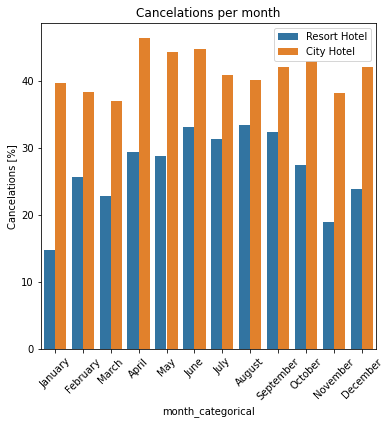
\includegraphics[width=0.8\textwidth]{img/TP2_KA_IB_files/TP2_KA_IB_29_0.png}

\end{col}

\begin{tcolorbox}

\textbf{Question 2.} Provide interpretation of the above plot.

\end{tcolorbox}

The cancelations at the City hotel are, in proportion, higher than in the Resort Hotel. For the Resort hotel, the cancelations are in proportion higher in Summer and Spring than in Winter and Fall. On the contrary, this seasonality is less clear for the City hotel. We only observe pics in April-May-June, then in September-October, and finally in December.

\begin{tcolorbox}

\textbf{Question 3.} What is the most and the second most common country of origin for reservations of each hotel?

\end{tcolorbox}

\begin{itemize}
\tightlist
\item
  \textbf{Resort Hotel} : the first most common country of origin for reservations is Portugal (PRT) and the second one is Great Britain (GBR)
\item
  \textbf{City Hotel} : the first most common country of origin for reservations is Portugal (PRT) and the second one is France (FRA)
\end{itemize}

See the plot below and the associated code in Annex \ref{annexe:annexe1}.

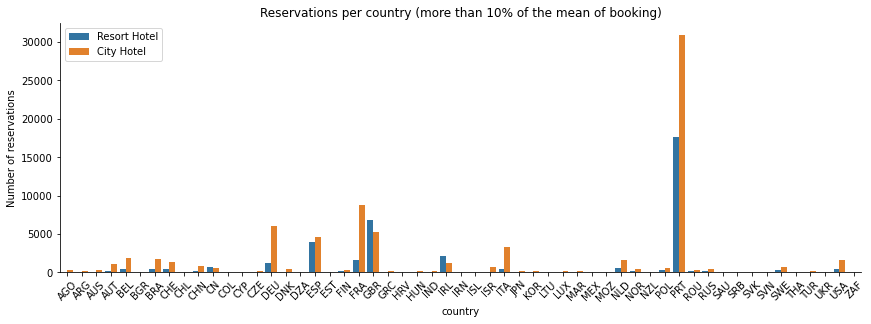
\includegraphics[width=0.8\textwidth]{img/TP2_KA_IB_files/TP2_KA_IB_36_1.png}

\begin{tcolorbox}

\textbf{Question 4.} Plot the number of cancelations for repeated and not repeated guests for both hotels.

\end{tcolorbox}

See the 2 following plots and the associated codes in Annex \ref{annexe:annexe1}.

\begin{col}{0.5\textwidth}

\centering

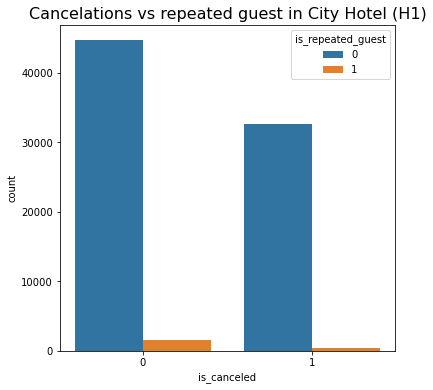
\includegraphics[width=0.7\textwidth]{img/TP2_KA_IB_files/TP2_KA_IB_41_1.png}

\end{col}

\begin{col}{0.5\textwidth}

\centering

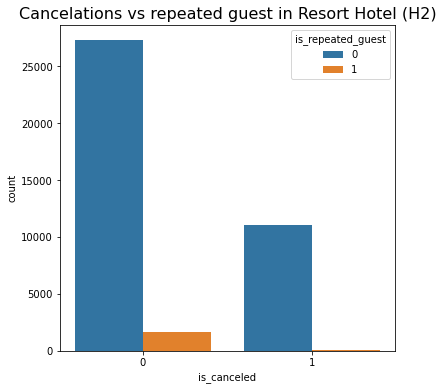
\includegraphics[width=0.7\textwidth]{img/TP2_KA_IB_files/TP2_KA_IB_42_1.png}

\end{col}

\begin{tcolorbox}

\textbf{Question 5.} Make the same plot for Resort Hotel. Make your conclusions.

\end{tcolorbox}

\begin{col}{0.5\textwidth}

\centering

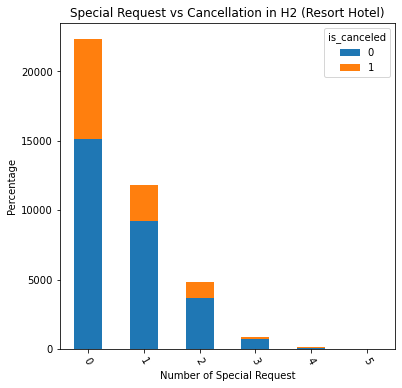
\includegraphics[width=0.7\textwidth]{img/TP2_KA_IB_files/TP2_KA_IB_49_1.png}

\end{col}

\begin{col}{0.5\textwidth}

\centering

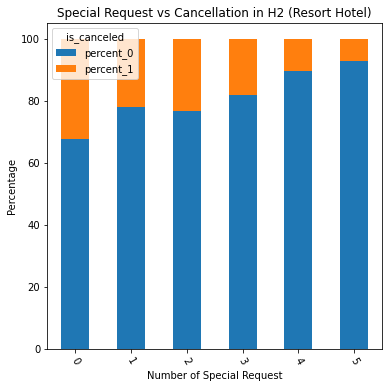
\includegraphics[width=0.7\textwidth]{img/TP2_KA_IB_files/TP2_KA_IB_51_1.png}

\end{col}

\newline

Most of the reservations in the Resort Hotel have no special request and the cancelation in this case is almost of 32 \%. However, when special requests are made, the cancelation rate is lower (22 \% when 1 special request is made, 23 \% when 2 special requests are made, 18 \% when 3 special request is made, 11 \% when 4 special request is made, 7 \% when 5 special request is made), but this decrease with the number of special requests is lower than with the City Hotel.

See the associated code in Annex \ref{annexe:annexe1}.

\hypertarget{predicting-cancellations-part-ii-ml}{%
\section{Predicting cancellations: Part II -- ML}\label{predicting-cancellations-part-ii-ml}}

\begin{tcolorbox}

\textbf{Question 1:} What is \texttt{OneHotEncoder()}? Why do we use it in our case?

\end{tcolorbox}

One-Hot-Encoding is a way (among others such as label encoding) to convert categorical values into numerical values because most of the ML algorithms work better with numerical inputs. In this strategy, each category value is converted into a new column and assigned a 1 or 0 (notation for true/false) value to the column. Let's consider the previous example of the names of the hotels (first column) with one-hot encoding (2 last columns).

\footnotesize

\begin{longtable}[]{@{}rlrr@{}}
\toprule
& hotel & 0 & 1\tabularnewline
\midrule
\endhead
0 & Resort Hotel & 0 & 1\tabularnewline
1 & Resort Hotel & 0 & 1\tabularnewline
2 & Resort Hotel & 0 & 1\tabularnewline
3 & Resort Hotel & 0 & 1\tabularnewline
4 & Resort Hotel & 0 & 1\tabularnewline
\bottomrule
\end{longtable}

\normalsize

We use it in our case because \textbf{many variables are categorical} : hotel, arrival\_date\_month, customer\_type, company, deposit\_type\dots

\emph{Source : see \href{https://towardsdatascience.com/categorical-encoding-using-label-encoding-and-one-hot-encoder-911ef77fb5bd}{here}.}

\begin{tcolorbox}

\textbf{Question 2:} In the previous example we again encounter the convergence problem. Of course we can set higher number of iterations, but it is time consuming. As you have seen, proper normalization can resolve the issue. Insert a normalization step in the pipeline. Note that we do not want to normalize the categorical data, it simply does not make sense. Be careful to normalize only the numerical data. Did it resolve the warning?

\end{tcolorbox}

To normalize the numeric features of the data, we modify the \texttt{numeric\_transformer}.

\begin{verbatim}
#numeric_transformer = SimpleImputer(strategy="constant", fill_value=0) # to deal with missing num data
\end{verbatim}

We change it into the following pipeline :

\begin{verbatim}
from sklearn.preprocessing import StandardScaler
numeric_transformer = Pipeline(steps=[
                                    ("imputer", SimpleImputer(strategy="constant", fill_value=0)),
                                    ("scaler", StandardScaler())]) #NEW : rescale the data !
\end{verbatim}

And it solved the warning! See the execution of the code in Annex \ref{annexe:annexe2}.

\begin{tcolorbox}

\textbf{Question 3:} As we can see, previous code uses only logistic regression. Modify the above code inserting your favorite ML method.

\end{tcolorbox}

Below, you can see the same actions but using the \textbf{SVM} method instead of logistic regressions. The main differences are:

\begin{itemize}
\tightlist
\item
  This time we use the following scaler : \texttt{MinMaxScaler()}
\item
  We use \texttt{LinearSVC()} instead of \texttt{LogisticRegression()}
\item
  We test the parameter \texttt{svc\_\_C} instead of \texttt{logreg\_\_C}
\end{itemize}

\begin{Shaded}
\begin{Highlighting}[]
\ImportTok{from}\NormalTok{ sklearn.svm }\ImportTok{import}\NormalTok{ LinearSVC}
\ImportTok{from}\NormalTok{ sklearn.preprocessing }\ImportTok{import}\NormalTok{ MinMaxScaler}
\NormalTok{numeric_transformer }\OperatorTok{=}\NormalTok{ Pipeline(steps}\OperatorTok{=}\NormalTok{[}
\NormalTok{                                    (}\StringTok{"imputer"}\NormalTok{, SimpleImputer(strategy}\OperatorTok{=}\StringTok{"constant"}\NormalTok{, fill_value}\OperatorTok{=}\DecValTok{0}\NormalTok{)),}
\NormalTok{                                    (}\StringTok{"scaler"}\NormalTok{, MinMaxScaler())]) }\CommentTok{#NEW : MinMaxScaler}
\NormalTok{preproc }\OperatorTok{=}\NormalTok{ ColumnTransformer(transformers}\OperatorTok{=}\NormalTok{[(}\StringTok{"num"}\NormalTok{, numeric_transformer, numeric_features),}
\NormalTok{                                          (}\StringTok{"cat"}\NormalTok{, categorical_transformer, categorical_features)])}
\NormalTok{models }\OperatorTok{=}\NormalTok{ [(}\StringTok{"logreg"}\NormalTok{, LogisticRegression(max_iter}\OperatorTok{=}\DecValTok{500}\NormalTok{)),}
\NormalTok{          (}\StringTok{"svc"}\NormalTok{, LinearSVC(max_iter}\OperatorTok{=}\DecValTok{700}\NormalTok{))]}
\NormalTok{grids }\OperatorTok{=}\NormalTok{ \{}\StringTok{"logreg"}\NormalTok{ : \{}\StringTok{'logreg__C'}\NormalTok{: np.logspace(}\OperatorTok{-}\DecValTok{2}\NormalTok{, }\DecValTok{2}\NormalTok{, }\DecValTok{5}\NormalTok{, base}\OperatorTok{=}\DecValTok{2}\NormalTok{)\},}
         \StringTok{"svc"}\NormalTok{ : \{}\StringTok{'svc__C'}\NormalTok{: np.logspace(}\OperatorTok{-}\DecValTok{2}\NormalTok{, }\DecValTok{2}\NormalTok{, }\DecValTok{5}\NormalTok{, base}\OperatorTok{=}\DecValTok{2}\NormalTok{)\}\}}
\ControlFlowTok{for}\NormalTok{ name, model }\KeywordTok{in}\NormalTok{ models:}
\NormalTok{    pipe }\OperatorTok{=}\NormalTok{ Pipeline(steps}\OperatorTok{=}\NormalTok{[(}\StringTok{'preprocessor'}\NormalTok{, preproc), (name, model)])}
\NormalTok{    clf }\OperatorTok{=}\NormalTok{ GridSearchCV(pipe, grids[name], cv}\OperatorTok{=}\DecValTok{3}\NormalTok{)}
\NormalTok{    clf.fit(X, y)}
    \BuiltInTok{print}\NormalTok{(}\StringTok{'Results for }\SpecialCharTok{\{\}}\StringTok{'}\NormalTok{.}\BuiltInTok{format}\NormalTok{(name))}
    \CommentTok{#print(clf.cv_results_)}
\NormalTok{    display(pd.DataFrame(clf.cv_results_)[[}\StringTok{'params'}\NormalTok{,}\StringTok{'mean_test_score'}\NormalTok{, }\StringTok{'std_test_score'}\NormalTok{,}
                                           \StringTok{'rank_test_score'}\NormalTok{]])}
\end{Highlighting}
\end{Shaded}

\begin{col}{0.5\textwidth}

\begin{verbatim}
Results for logreg
\end{verbatim}

\footnotesize

\begin{longtable}[]{@{}rlrrr@{}}
\toprule
& params & mean\_test\_score & std\_test\_score & rank\_test\_score\tabularnewline
\midrule
\endhead
0 & \{'logreg\_\_C': 0.25\} & 0.73992 & 0.0330775 & 1\tabularnewline
1 & \{'logreg\_\_C': 0.5\} & 0.739283 & 0.0336877 & 2\tabularnewline
2 & \{'logreg\_\_C': 1.0\} & 0.734693 & 0.0391517 & 3\tabularnewline
3 & \{'logreg\_\_C': 2.0\} & 0.731133 & 0.0435457 & 4\tabularnewline
4 & \{'logreg\_\_C': 4.0\} & 0.72785 & 0.0476724 & 5\tabularnewline
\bottomrule
\end{longtable}

\end{col}

\begin{col}{0.5\textwidth}

\begin{verbatim}
Results for svc
\end{verbatim}

\footnotesize

\begin{longtable}[]{@{}rlrrr@{}}
\toprule
& params & mean\_test\_score & std\_test\_score & rank\_test\_score\tabularnewline
\midrule
\endhead
0 & \{'svc\_\_C': 0.25\} & 0.740933 & 0.0362662 & 1\tabularnewline
1 & \{'svc\_\_C': 0.5\} & 0.738647 & 0.0392476 & 2\tabularnewline
2 & \{'svc\_\_C': 1.0\} & 0.737424 & 0.0408303 & 3\tabularnewline
3 & \{'svc\_\_C': 2.0\} & 0.735489 & 0.0434047 & 4\tabularnewline
4 & \{'svc\_\_C': 4.0\} & 0.734057 & 0.0453227 & 5\tabularnewline
\bottomrule
\end{longtable}

\end{col}

\newline

\textbf{\faArrowCircleRight{} The results of SVM seem to be a bit better than the ones for the logistic regression : the mean test scores are globally higher.}

\hypertarget{the-homework-part-iii}{%
\section{The homework: Part III}\label{the-homework-part-iii}}

\hypertarget{first-step-choose-the-relevant-features-and-build-the-dataset}{%
\subsection{FIRST STEP : choose the relevant features and build the dataset}\label{first-step-choose-the-relevant-features-and-build-the-dataset}}

\begin{col}{0.4\textwidth}

See in Annex \ref{annexe:annexe5} the whole code for Part III.

\medskip

We first \textbf{delete} from the dataset \textbf{4 features} that cannot be observed at the moment when the SMS is sent :\texttt{is\_canceled}, \texttt{assigned\_room\_type}, \texttt{reservation\_status} and \texttt{reservation\_status\_date}. See in Annex \ref{annexe:annexe3} for more details about these variables.

\medskip

Then, we look at the features containing lots of missing data (see figure on the right). The feature ``company'' displays a lot of missing data. Therefore we don't use this feature in our predicting models.

\medskip

Finally, we create the data.frame we need by creating a binary variable called \texttt{bool\_parking} whose value is 1 if \texttt{required\_car\_parking\_spaces} \textgreater{} 0

\end{col}

\begin{col}{0.6\textwidth}

\centering

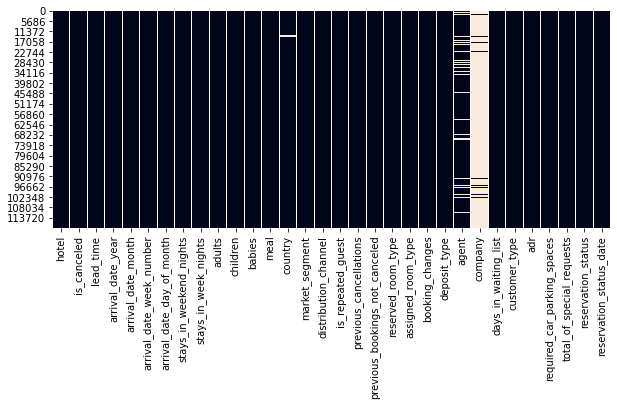
\includegraphics[width=1\textwidth]{img/TP2_KA_IB_files/TP2_KA_IB_76_1.png}

\end{col}

\hypertarget{second-step-exploratory-data-analysis}{%
\subsection{SECOND STEP : Exploratory Data analysis}\label{second-step-exploratory-data-analysis}}

Now, we do some plots to see what kind of variables seem to be important to predict the outcome \texttt{bool\_parking}. Two examples of the plots are put below. The rest of them are available in Annex \ref{annexe:annexe4}.

\begin{col}{0.6\textwidth}

\centering

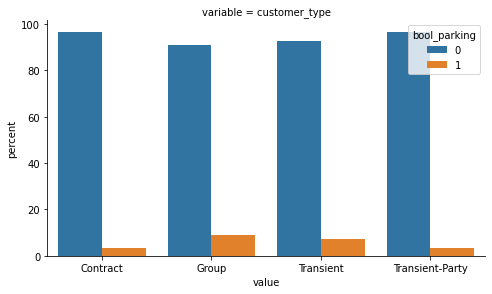
\includegraphics[width=1\textwidth]{img/TP2_KA_IB_files/TP2_KA_IB_80_6.png}

\end{col}

\begin{col}{0.4\textwidth}

\centering

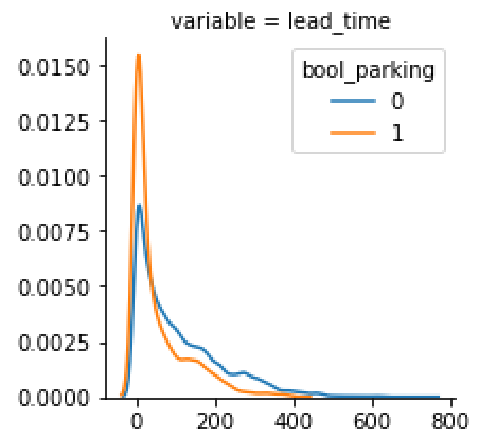
\includegraphics[width=0.8\textwidth]{img/TP2_KA_IB_files/lead_time.png}

\end{col}

\newline

These plots make us draw some first conclusions about the interesting predictors of the outcome. People more susceptible to use a parking seem to be people :

\begin{itemize}
\tightlist
\item
  coming in groups and transient travellers : guests who are predominantly on-the-move and seek short hotel-stays (\texttt{customer\_type\ =\ Group} or \texttt{Transient})
\item
  going to the Resort Hotel (\texttt{hotel\ =\ Resort\ Hotel}) \faArrowCircleRight{} It may mean that we should do 2 different predictive models, one for each hotel
\item
  who book directly at the hotel (\texttt{market\_segment\ =\ direct})
\item
  who book a certain kind of room (\texttt{reserved\_room\_type\ =\ H}) but for anonymity reasons we don't know what it represents
\item
  coming in the summer (\texttt{arrival\_date\_week\_number} around \texttt{25})
\item
  who don't book in advance (\texttt{lead\_time} close to \texttt{0})
\item
  rich (\texttt{adr} is \texttt{high})
\item
  who have children (children is \texttt{high})
\end{itemize}

\hypertarget{third-step-modelisation}{%
\subsection{THIRD STEP : Modelisation}\label{third-step-modelisation}}

Now that the data-processing is done, we apply some ML models to predict the variable \texttt{bool\_parking}.

\hypertarget{models-including-all-the-variables}{%
\subsubsection{Models including all the variables}\label{models-including-all-the-variables}}

After preparing, the test and training set, we run the models (SVM and logistic regressions) using Cross-validation. Finally, we run the models with the best parameters and evaluate them with different scores. Below are the results.

\begin{col}{0.5\textwidth}

\footnotesize

\begin{verbatim}
Results for logreg
Returned hyperparameter: {'logreg__C': 0.25}
Best classification accuracy in train is: 0.9374483437555715
Classification accuracy on test is: 0.9391584025730367
\end{verbatim}

\begin{longtable}[]{@{}rlrrr@{}}
\toprule
& params & mean\_test\_score & std\_test\_score & rank\_test\_score\tabularnewline
\midrule
\endhead
0 & \{'logreg\_\_C': 0.25\} & 0.937996 & 1.53278e-05 & 2\tabularnewline
1 & \{'logreg\_\_C': 0.5\} & 0.938018 & 9.78925e-07 & 1\tabularnewline
2 & \{'logreg\_\_C': 1.0\} & 0.937996 & 3.20887e-05 & 3\tabularnewline
3 & \{'logreg\_\_C': 2.0\} & 0.937996 & 3.20887e-05 & 3\tabularnewline
4 & \{'logreg\_\_C': 4.0\} & 0.937984 & 4.78791e-05 & 5\tabularnewline
\bottomrule
\end{longtable}

\begin{verbatim}
MSE logreg:  0.25110316775715696
R2 logreg:  -0.08354580290869595
accuracy logreg :  0.936947199142321
\end{verbatim}

\end{col}

\begin{col}{0.5\textwidth}

\footnotesize

\begin{verbatim}
Results for svc
Returned hyperparameter: {'svc__C': 0.25}
Best classification accuracy in train is: 0.9374483482455481
Classification accuracy on test is: 0.9391584025730367
\end{verbatim}

\begin{longtable}[]{@{}rlrrr@{}}
\toprule
& params & mean\_test\_score & std\_test\_score & rank\_test\_score\tabularnewline
\midrule
\endhead
0 & \{'svc\_\_C': 0.25\} & 0.93804 & 1.48151e-05 & 1\tabularnewline
1 & \{'svc\_\_C': 0.5\} & 0.93804 & 1.48151e-05 & 1\tabularnewline
2 & \{'svc\_\_C': 1.0\} & 0.93804 & 1.48151e-05 & 1\tabularnewline
3 & \{'svc\_\_C': 2.0\} & 0.93804 & 1.48151e-05 & 1\tabularnewline
4 & \{'svc\_\_C': 4.0\} & 0.93804 & 1.48151e-05 & 1\tabularnewline
\bottomrule
\end{longtable}

\begin{verbatim}
MSE svc:  0.25210185856501033
R2 svc:  -0.06839376846142531
accuracy svc :  0.9364446529080676
\end{verbatim}

\end{col}

\newline

\textbf{\faArrowCircleRight{} Both SVM and LogisticRegression WITHOUT selection of features present really performent results. The accuracy is nearly 94\%. Indeed, the number of individuals is +100 000 (n) and the number of features (p) is around 30. Therefore, we have n \textgreater{}\textgreater{} p which prevents from overfitting}

\hypertarget{models-with-best-predictive-features-chosen-manually}{%
\subsubsection{Models with best predictive features chosen MANUALLY}\label{models-with-best-predictive-features-chosen-manually}}

Now we try to pick up \textbf{MANUALLY} features with high predicting powers to see if it can reduce over-fitting and show better results. We filter columns with the 8 pre-selected variables (4 numeric features : ``arrival\_date\_week\_number'',``lead\_time'', ``adr'',``children'' and 4 categorical features ``customer\_type'',``hotel'', ``market\_segment'', ``reserved\_room\_type'') and we do the same process as before.

\begin{col}{0.5\textwidth}

\footnotesize

\begin{verbatim}
Results for logreg
Returned hyperparameter: {'logreg__C': 2.0}
Best classification accuracy in train is: 0.9379620748954963
Classification accuracy on test is: 0.9375502546234253
\end{verbatim}

\begin{longtable}[]{@{}rlrrr@{}}
\toprule
& params & mean\_test\_score & std\_test\_score & rank\_test\_score\tabularnewline
\midrule
\endhead
0 & \{'logreg\_\_C': 0.25\} & 0.937783 & 2.82109e-05 & 1\tabularnewline
1 & \{'logreg\_\_C': 0.5\} & 0.937772 & 1.63076e-05 & 3\tabularnewline
2 & \{'logreg\_\_C': 1.0\} & 0.937783 & 2.82109e-05 & 1\tabularnewline
3 & \{'logreg\_\_C': 2.0\} & 0.937772 & 4.25343e-05 & 4\tabularnewline
4 & \{'logreg\_\_C': 4.0\} & 0.937772 & 4.25343e-05 & 4\tabularnewline
\bottomrule
\end{longtable}

\begin{verbatim}
MSE logreg:  0.246864551270153
R2 logreg:  -0.06660949113779324
accuracy logreg :  0.939057893326186
\end{verbatim}

\end{col}

\begin{col}{0.5\textwidth}

\footnotesize

\begin{verbatim}
Results for svc
Returned hyperparameter: {'svc__C': 0.25}
Best classification accuracy in train is: 0.9379844099095207
Classification accuracy on test is: 0.9375502546234253
\end{verbatim}

\begin{longtable}[]{@{}rlrrr@{}}
\toprule
& params & mean\_test\_score & std\_test\_score & rank\_test\_score\tabularnewline
\midrule
\endhead
0 & \{'svc\_\_C': 0.25\} & 0.937795 & 1.53264e-05 & 1\tabularnewline
1 & \{'svc\_\_C': 0.5\} & 0.937795 & 1.53264e-05 & 1\tabularnewline
2 & \{'svc\_\_C': 1.0\} & 0.937795 & 1.53264e-05 & 1\tabularnewline
3 & \{'svc\_\_C': 2.0\} & 0.937795 & 1.53264e-05 & 1\tabularnewline
4 & \{'svc\_\_C': 4.0\} & 0.937795 & 1.53264e-05 & 1\tabularnewline
\bottomrule
\end{longtable}

\begin{verbatim}
MSE svc:  0.246864551270153
R2 svc:  -0.06489707089086316
accuracy svc :  0.939057893326186
\end{verbatim}

\end{col}

\newline

\textbf{\faArrowCircleRight{} Both SVM and LogisticRegression WITH MANUAL selection of features still present really good results. Even if the different scores are a bit less promising than the ones of the previous method, they are still very good. For example, the accuracy is here still nearly 94\%.}

\hypertarget{models-with-best-predictive-features-chosen-with-regularized-regressions}{%
\subsubsection{Models with best predictive features chosen with REGULARIZED REGRESSIONS}\label{models-with-best-predictive-features-chosen-with-regularized-regressions}}

We try to improve the models using a polynomial regression with a regularization called LASSO. This method only selects the features that best predict the outcome. Indeed, as we explained earlier, subsetting the features may prevent from overfitting. LASSO regression is such as \(\hat f = \underset{f \in \mathcal F_n^\text{poly}}{argmin} \{ \frac{1}{2m} \sum_{i=1}^m (Y_i - f(X_i))^2 + \alpha \sum_{k=1}^n | a_k | \}\) where \(\alpha\) \textgreater{} 0 is a parameter to chose.

\begin{itemize}
\tightlist
\item
  If \(\alpha\) is too large, all the coefficients of the regression equal to zero
\item
  If \(\alpha\) is too small and close to 0, we get the coefficients of the usual linear regression.
\end{itemize}

Thus, we must find a compromise, by choosing alpha by cross-validation.

The ``lasso path'' can also help us. This is a graph that relates the value of \(\alpha\) to the estimated coefficients.

\begin{col}{0.5\textwidth}

\centering

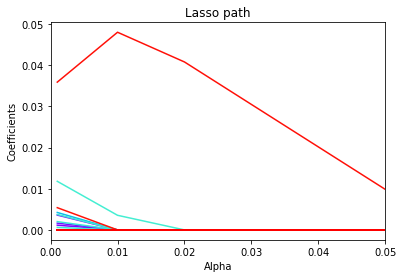
\includegraphics[width=1\textwidth]{img/TP2_KA_IB_files/TP2_KA_IB_101_1.png}

\end{col}

\begin{col}{0.5\textwidth}

\centering

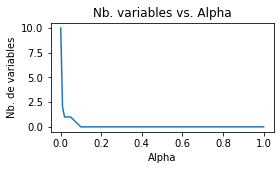
\includegraphics[width=1\textwidth]{img/TP2_KA_IB_files/TP2_KA_IB_102_0.png}

\end{col}

\begin{col}{0.5\textwidth}

\footnotesize

\begin{longtable}[]{@{}rlr@{}}
\toprule
& Variables & Coefficients\tabularnewline
\midrule
\endhead
3 & arrival\_date\_week\_number & 6.61727e-06\tabularnewline
15 & meal\_BB & 0.00188516\tabularnewline
156 & country\_SLV & 0.00252614\tabularnewline
209 & distribution\_channel\_GDS & 0.00402931\tabularnewline
212 & hotel\_Resort Hotel & 0.000188013\tabularnewline
213 & reserved\_room\_type\_A & 0.00470136\tabularnewline
223 & deposit\_type\_Non Refund & 0.0174298\tabularnewline
562 & customer\_type\_Contract & 0.00601914\tabularnewline
564 & is\_repeated\_guest\_0 & 0.032911\tabularnewline
\bottomrule
\end{longtable}

\end{col}

\begin{col}{0.5\textwidth}

\footnotesize

alpha MSE
0 1.000 0.061803
1 0.800 0.061803
2 0.500 0.061803
3 0.250 0.061803
4 0.100 0.061803
5 0.050 0.060326
6 0.025 0.056838
7 0.020 0.056129
8 0.010 0.055185
9 0.001 0.052854
best alpha: 0.001

\end{col}

\newline

The best alpha is the lowest (0.001). It is logical because, as we said earlier, the number of features is low (p=30) compared to the number of individuals (n=+100 000). Therefore, regularized regressions are not necessary in our case. Finally, we run the lasso with the best \(\alpha\) and evaluate it with different scores.

\begin{verbatim}
MSE lasso:  0.23160623528346608
R2 lasso:  -0.06815575882526304
\end{verbatim}

\textbf{\faArrowCircleRight{} We can see that the MSE obtained on the test set (0.23) is lower (and thus better) than the one of the previous models (0.25), which means that the regularization may have improved a little bit the model !}

\clearpage

\newpage

\hypertarget{appendix-appendix}{%
\appendix}


\addtocontents{toc}{\protect\setcounter{tocdepth}{1}}
\setcounter{page}{0}
\pagenumbering{roman}

\hypertarget{annexe:annexe1}{%
\section{Code of Part I}\label{annexe:annexe1}}

\hypertarget{question-3}{%
\subsection{Question 3}\label{question-3}}

\begin{Shaded}
\begin{Highlighting}[]
\CommentTok{# Lets create a database following the same model than before but using countries instead of months}
\CommentTok{#First Hotel}
\NormalTok{n2_reserv_H1 }\OperatorTok{=}\NormalTok{ data.loc[(data[}\StringTok{"hotel"}\NormalTok{] }\OperatorTok{==} \StringTok{"Resort Hotel"}\NormalTok{)].groupby(}\StringTok{"country"}\NormalTok{)[}\StringTok{"hotel"}\NormalTok{].count()}
\NormalTok{data2_visualH1 }\OperatorTok{=}\NormalTok{ pd.DataFrame(\{}\StringTok{"hotel"}\NormalTok{: }\StringTok{"Resort Hotel"}\NormalTok{,}
                                \StringTok{"country"}\NormalTok{: }\BuiltInTok{list}\NormalTok{(n2_reserv_H1.index),}
                                \StringTok{"n_booking"}\NormalTok{: }\BuiltInTok{list}\NormalTok{(n2_reserv_H1.values)\})}
\NormalTok{data2_visualH1.sort_values(by}\OperatorTok{=}\NormalTok{[}\StringTok{'n_booking'}\NormalTok{], ascending}\OperatorTok{=}\VariableTok{False}\NormalTok{)}
\end{Highlighting}
\end{Shaded}

\begin{longtable}[]{@{}rllr@{}}
\toprule
& hotel & country & n\_booking\tabularnewline
\midrule
\endhead
95 & Resort Hotel & PRT & 17630\tabularnewline
45 & Resort Hotel & GBR & 6814\tabularnewline
40 & Resort Hotel & ESP & 3957\tabularnewline
55 & Resort Hotel & IRL & 2166\tabularnewline
44 & Resort Hotel & FRA & 1611\tabularnewline
\bottomrule
\end{longtable}

\begin{Shaded}
\begin{Highlighting}[]
\CommentTok{#Second Hotel}
\NormalTok{n2_reserv_H2 }\OperatorTok{=}\NormalTok{ data.loc[(data[}\StringTok{"hotel"}\NormalTok{] }\OperatorTok{==} \StringTok{"City Hotel"}\NormalTok{)].groupby(}\StringTok{"country"}\NormalTok{)[}\StringTok{"hotel"}\NormalTok{].count()}
\NormalTok{data2_visualH2 }\OperatorTok{=}\NormalTok{ pd.DataFrame(\{}\StringTok{"hotel"}\NormalTok{: }\StringTok{"City Hotel"}\NormalTok{,}
                                \StringTok{"country"}\NormalTok{: }\BuiltInTok{list}\NormalTok{(n2_reserv_H2.index),}
                                \StringTok{"n_booking"}\NormalTok{: }\BuiltInTok{list}\NormalTok{(n2_reserv_H2.values)\})}
\NormalTok{data2_visualH2.sort_values(by}\OperatorTok{=}\NormalTok{[}\StringTok{'n_booking'}\NormalTok{], ascending}\OperatorTok{=}\VariableTok{False}\NormalTok{)}
\end{Highlighting}
\end{Shaded}

\begin{longtable}[]{@{}rllr@{}}
\toprule
& hotel & country & n\_booking\tabularnewline
\midrule
\endhead
125 & City Hotel & PRT & 30960\tabularnewline
50 & City Hotel & FRA & 8804\tabularnewline
39 & City Hotel & DEU & 6084\tabularnewline
53 & City Hotel & GBR & 5315\tabularnewline
46 & City Hotel & ESP & 4611\tabularnewline
\bottomrule
\end{longtable}

\begin{Shaded}
\begin{Highlighting}[]
\NormalTok{data2_visual }\OperatorTok{=}\NormalTok{ pd.concat([data2_visualH1, data2_visualH2], ignore_index}\OperatorTok{=}\VariableTok{True}\NormalTok{)}
\NormalTok{data2_visual }\OperatorTok{=}\NormalTok{ data2_visual.sort_values(by}\OperatorTok{=}\NormalTok{[}\StringTok{'country'}\NormalTok{], ascending}\OperatorTok{=}\VariableTok{True}\NormalTok{)}

\NormalTok{plt.figure(figsize}\OperatorTok{=}\NormalTok{(}\DecValTok{6}\NormalTok{, }\DecValTok{6}\NormalTok{))}
\CommentTok{#sns.barplot(x = "country", y = "n_booking" , hue="hotel",}
\CommentTok{#            hue_order = ["Resort Hotel", "City Hotel"], data=data2_visual)}
\NormalTok{sns.catplot(x }\OperatorTok{=} \StringTok{"country"}\NormalTok{, y }\OperatorTok{=} \StringTok{"n_booking"}\NormalTok{ , hue}\OperatorTok{=}\StringTok{"hotel"}\NormalTok{, hue_order }\OperatorTok{=}\NormalTok{ [}\StringTok{"Resort Hotel"}\NormalTok{, }\StringTok{"City Hotel"}\NormalTok{],}
\NormalTok{            data}\OperatorTok{=}\NormalTok{data2_visual[data2_visual[}\StringTok{"n_booking"}\NormalTok{]}\OperatorTok{>}\NormalTok{(}\FloatTok{0.1}\OperatorTok{*}\NormalTok{np.mean(data2_visual[}\StringTok{"n_booking"}\NormalTok{]))],}
\NormalTok{            legend_out}\OperatorTok{=}\VariableTok{False}\NormalTok{, kind}\OperatorTok{=}\StringTok{"bar"}\NormalTok{, height }\OperatorTok{=} \DecValTok{4}\NormalTok{, aspect}\OperatorTok{=}\DecValTok{3}\NormalTok{)}
\NormalTok{plt.title(}\StringTok{"Reservations per country (more than 10}\SpecialCharTok{% o}\StringTok{f the mean of booking)"}\NormalTok{)}
\NormalTok{plt.xticks(rotation}\OperatorTok{=}\DecValTok{45}\NormalTok{)}
\NormalTok{plt.ylabel(}\StringTok{"Number of reservations"}\NormalTok{)}
\NormalTok{plt.legend()}
\NormalTok{plt.show()}
\end{Highlighting}
\end{Shaded}

\hypertarget{question-4}{%
\subsection{Question 4}\label{question-4}}

\begin{Shaded}
\begin{Highlighting}[]
\CommentTok{# The same only with City Hotel (H1)}
\NormalTok{plt.figure(figsize}\OperatorTok{=}\NormalTok{(}\DecValTok{6}\NormalTok{, }\DecValTok{6}\NormalTok{))}
\NormalTok{sns.countplot(x}\OperatorTok{=}\StringTok{"is_canceled"}\NormalTok{, hue}\OperatorTok{=}\StringTok{'is_repeated_guest'}\NormalTok{, data}\OperatorTok{=}\NormalTok{data[(data[}\StringTok{'hotel'}\NormalTok{] }\OperatorTok{==} \StringTok{'City Hotel'}\NormalTok{)])}
\NormalTok{plt.title(}\StringTok{"Cancelations vs repeated guest in City Hotel (H1)"}\NormalTok{, fontsize}\OperatorTok{=}\DecValTok{16}\NormalTok{)}
\NormalTok{plt.plot()}
\end{Highlighting}
\end{Shaded}

\begin{Shaded}
\begin{Highlighting}[]
\CommentTok{# The same only with Resort Hotel (H2)}
\NormalTok{plt.figure(figsize}\OperatorTok{=}\NormalTok{(}\DecValTok{6}\NormalTok{, }\DecValTok{6}\NormalTok{))}
\NormalTok{sns.countplot(x}\OperatorTok{=}\StringTok{"is_canceled"}\NormalTok{, hue}\OperatorTok{=}\StringTok{'is_repeated_guest'}\NormalTok{, data}\OperatorTok{=}\NormalTok{data[(data[}\StringTok{'hotel'}\NormalTok{] }\OperatorTok{==} \StringTok{'Resort Hotel'}\NormalTok{)])}
\NormalTok{plt.title(}\StringTok{"Cancelations vs repeated guest in Resort Hotel (H2)"}\NormalTok{, fontsize}\OperatorTok{=}\DecValTok{16}\NormalTok{)}
\NormalTok{plt.plot()}
\end{Highlighting}
\end{Shaded}

\hypertarget{question-5}{%
\subsection{Question 5}\label{question-5}}

\begin{Shaded}
\begin{Highlighting}[]
\NormalTok{data_req2 }\OperatorTok{=}\NormalTok{ data[(data[}\StringTok{'hotel'}\NormalTok{] }\OperatorTok{==} \StringTok{'Resort Hotel'}\NormalTok{)].groupby([}\StringTok{'total_of_special_requests'}\NormalTok{,}
                                                             \StringTok{'is_canceled'}\NormalTok{]).size().unstack(level}\OperatorTok{=}\DecValTok{1}\NormalTok{)}
\NormalTok{data_req2.plot(kind}\OperatorTok{=}\StringTok{'bar'}\NormalTok{, stacked}\OperatorTok{=}\VariableTok{True}\NormalTok{, figsize}\OperatorTok{=}\NormalTok{(}\DecValTok{6}\NormalTok{,}\DecValTok{6}\NormalTok{))}
\NormalTok{plt.title(}\StringTok{'Special Request vs Cancellation in H2 (Resort Hotel)'}\NormalTok{)}
\NormalTok{plt.xlabel(}\StringTok{'Number of Special Request'}\NormalTok{, fontsize}\OperatorTok{=}\DecValTok{10}\NormalTok{)}
\NormalTok{plt.xticks(rotation}\OperatorTok{=}\DecValTok{300}\NormalTok{)}
\NormalTok{plt.ylabel(}\StringTok{'Percentage'}\NormalTok{, fontsize}\OperatorTok{=}\DecValTok{10}\NormalTok{)}
\end{Highlighting}
\end{Shaded}

\begin{Shaded}
\begin{Highlighting}[]
\CommentTok{# From raw value to percentage}
\NormalTok{total }\OperatorTok{=}\NormalTok{ [i}\OperatorTok{+}\NormalTok{j }\ControlFlowTok{for}\NormalTok{ i,j }\KeywordTok{in} \BuiltInTok{zip}\NormalTok{(data_req2[}\DecValTok{0}\NormalTok{], data_req2[}\DecValTok{1}\NormalTok{])]}
\NormalTok{data_req2[}\StringTok{'percent_0'}\NormalTok{] }\OperatorTok{=}\NormalTok{ [i }\OperatorTok{/}\NormalTok{ j }\OperatorTok{*} \DecValTok{100} \ControlFlowTok{for}\NormalTok{ i,j }\KeywordTok{in} \BuiltInTok{zip}\NormalTok{(data_req2[}\DecValTok{0}\NormalTok{], total)]}
\NormalTok{data_req2[}\StringTok{'percent_1'}\NormalTok{] }\OperatorTok{=}\NormalTok{ [i }\OperatorTok{/}\NormalTok{ j }\OperatorTok{*} \DecValTok{100} \ControlFlowTok{for}\NormalTok{ i,j }\KeywordTok{in} \BuiltInTok{zip}\NormalTok{(data_req2[}\DecValTok{1}\NormalTok{], total)]}
\NormalTok{data_req2.iloc[:, }\DecValTok{2}\NormalTok{:}\DecValTok{4}\NormalTok{]}
\end{Highlighting}
\end{Shaded}

\begin{longtable}[]{@{}rrrrr@{}}
\toprule
total\_of\_special\_requests & 0 & 1 & percent\_0 & percent\_1\tabularnewline
\midrule
\endhead
0 & 15145 & 7216 & 67.7295 & 32.2705\tabularnewline
1 & 9209 & 2597 & 78.0027 & 21.9973\tabularnewline
2 & 3700 & 1127 & 76.6522 & 23.3478\tabularnewline
3 & 744 & 166 & 81.7582 & 18.2418\tabularnewline
4 & 127 & 15 & 89.4366 & 10.5634\tabularnewline
5 & 13 & 1 & 92.8571 & 7.14286\tabularnewline
\bottomrule
\end{longtable}

\begin{Shaded}
\begin{Highlighting}[]
\NormalTok{data_req2.iloc[:, }\DecValTok{2}\NormalTok{:}\DecValTok{4}\NormalTok{].plot(kind}\OperatorTok{=}\StringTok{'bar'}\NormalTok{, stacked}\OperatorTok{=}\VariableTok{True}\NormalTok{, figsize}\OperatorTok{=}\NormalTok{(}\DecValTok{6}\NormalTok{,}\DecValTok{6}\NormalTok{))}
\NormalTok{plt.title(}\StringTok{'Special Request vs Cancellation in H1 (Resort Hotel)'}\NormalTok{)}
\NormalTok{plt.xlabel(}\StringTok{'Number of Special Request'}\NormalTok{, fontsize}\OperatorTok{=}\DecValTok{10}\NormalTok{)}
\NormalTok{plt.xticks(rotation}\OperatorTok{=}\DecValTok{300}\NormalTok{)}
\NormalTok{plt.ylabel(}\StringTok{'Percentage'}\NormalTok{, fontsize}\OperatorTok{=}\DecValTok{10}\NormalTok{)}
\end{Highlighting}
\end{Shaded}

\newpage

\hypertarget{annexe:annexe2}{%
\section{Code of Part II}\label{annexe:annexe2}}

\hypertarget{question-1}{%
\subsection{Question 1}\label{question-1}}

\begin{Shaded}
\begin{Highlighting}[]
\ImportTok{import}\NormalTok{ pandas }\ImportTok{as}\NormalTok{ pd}
\ImportTok{import}\NormalTok{ numpy }\ImportTok{as}\NormalTok{ np}
\ImportTok{from}\NormalTok{ sklearn.preprocessing }\ImportTok{import}\NormalTok{ OneHotEncoder }
\CommentTok{# creating instance of one-hot-encoder}
\NormalTok{enc }\OperatorTok{=}\NormalTok{ OneHotEncoder(handle_unknown}\OperatorTok{=}\StringTok{'ignore'}\NormalTok{)}
\CommentTok{# passing hotel-types-cat column (label encoded values of bridge_types)}
\NormalTok{enc_df }\OperatorTok{=}\NormalTok{ pd.DataFrame(enc.fit_transform(data[[}\StringTok{'hotel'}\NormalTok{]]).toarray())}
\CommentTok{# merge with main dataframe on key values}
\NormalTok{hotel_df }\OperatorTok{=}\NormalTok{ data.iloc[:, }\DecValTok{0}\NormalTok{:}\DecValTok{1}\NormalTok{].join(enc_df)}
\NormalTok{hotel_df.head()}
\end{Highlighting}
\end{Shaded}

\hypertarget{question-2}{%
\subsection{Question 2}\label{question-2}}

\begin{Shaded}
\begin{Highlighting}[]
\ImportTok{from}\NormalTok{ sklearn.preprocessing }\ImportTok{import}\NormalTok{ StandardScaler}
\CommentTok{#numeric_transformer = SimpleImputer(strategy="constant", fill_value=0) # to deal with missing numeric data}
\NormalTok{numeric_transformer }\OperatorTok{=}\NormalTok{ Pipeline(steps}\OperatorTok{=}\NormalTok{[}
\NormalTok{                                    (}\StringTok{"imputer"}\NormalTok{, SimpleImputer(strategy}\OperatorTok{=}\StringTok{"constant"}\NormalTok{, fill_value}\OperatorTok{=}\DecValTok{0}\NormalTok{)),}
\NormalTok{                                    (}\StringTok{"scaler"}\NormalTok{, StandardScaler())]) }\CommentTok{#NEW : rescale the data !}
\NormalTok{preproc }\OperatorTok{=}\NormalTok{ ColumnTransformer(transformers}\OperatorTok{=}\NormalTok{[(}\StringTok{"num"}\NormalTok{, numeric_transformer, numeric_features),}
\NormalTok{                                          (}\StringTok{"cat"}\NormalTok{, categorical_transformer, categorical_features)])}
\end{Highlighting}
\end{Shaded}

\begin{Shaded}
\begin{Highlighting}[]
\NormalTok{models }\OperatorTok{=}\NormalTok{ [(}\StringTok{"logreg"}\NormalTok{, LogisticRegression(max_iter}\OperatorTok{=}\DecValTok{500}\NormalTok{))]}
\NormalTok{grids }\OperatorTok{=}\NormalTok{ \{}\StringTok{"logreg"}\NormalTok{ : \{}\StringTok{'logreg__C'}\NormalTok{: np.logspace(}\OperatorTok{-}\DecValTok{2}\NormalTok{, }\DecValTok{2}\NormalTok{, }\DecValTok{5}\NormalTok{, base}\OperatorTok{=}\DecValTok{2}\NormalTok{)\}\}}
\ControlFlowTok{for}\NormalTok{ name, model }\KeywordTok{in}\NormalTok{ models:}
\NormalTok{    pipe }\OperatorTok{=}\NormalTok{ Pipeline(steps}\OperatorTok{=}\NormalTok{[(}\StringTok{'preprocessor'}\NormalTok{, preproc), (name, model)])}
\NormalTok{    clf }\OperatorTok{=}\NormalTok{ GridSearchCV(pipe, grids[name], cv}\OperatorTok{=}\DecValTok{3}\NormalTok{)}
\NormalTok{    clf.fit(X, y)}
    \BuiltInTok{print}\NormalTok{(}\StringTok{'Results for }\SpecialCharTok{\{\}}\StringTok{'}\NormalTok{.}\BuiltInTok{format}\NormalTok{(name))}
    \BuiltInTok{print}\NormalTok{(clf.cv_results_)}
\end{Highlighting}
\end{Shaded}

\begin{verbatim}
Results for logreg
{'mean_fit_time': array([1.07707651, 1.06985847, 1.26302139, 0.94357912, 1.00347384]),
'std_fit_time': array([0.22217166, 0.14027325, 0.44600286, 0.12203947, 0.05911086]),
'mean_score_time': array([0.0600067 , 0.0611678 , 0.05684272, 0.0552206 ,
0.06061093]), 'std_score_time': array([0.00130701, 0.0016936 , 0.00354926, 0.00281719,
0.00184487]), 'param_logreg__C': masked_array(data=[0.25, 0.5, 1.0, 2.0, 4.0],
             mask=[False, False, False, False, False],
       fill_value='?',
            dtype=object), 'params': [{'logreg__C': 0.25}, {'logreg__C': 0.5},
            {'logreg__C': 1.0}, {'logreg__C': 2.0}, {'logreg__C': 4.0}],
            'split0_test_score': array([0.70128402, 0.7000779 , 0.68552906,
            0.67786517, 0.66600498]), 'split1_test_score': array([0.78262181,
            0.78244591, 0.78232028, 0.78221977, 0.78219464]),
            'split2_test_score': array([0.73585285, 0.73582772, 0.73582772,
            0.736079  , 0.736079  ]), 'mean_test_score': array([0.73991956,
            0.73945051, 0.73455902, 0.73205464, 0.72809287]),
            'std_test_score': array([0.03333029, 0.03372404, 0.03952503,
            0.04269752, 0.04776919]),
            'rank_test_score': array([1, 2, 3, 4, 5])}
\end{verbatim}

\newpage

\hypertarget{annexe:annexe3}{%
\section{Variables observed when sending the SMS}\label{annexe:annexe3}}

The variables deleted from the dataset because they cannot be observed at the moment when the SMS is sent are in a strikethrough font below with their definitions.

-\textbf{hotel} : Hotel (H1 = Resort Hotel or H2 = City Hotel)

-\sout{\textbf{is\_canceled} : Value indicating if the booking was canceled (1) or not (0)}

-\textbf{lead\_time} : Number of days that elapsed between the entering date of the booking into the PMS and the arrival date

-\textbf{arrival\_date\_year} : Year of arrival date

-\textbf{arrival\_date\_month} : Month of arrival date

-\textbf{arrival\_date\_week\_number} : Week number of year for arrival date

-\textbf{arrival\_date\_day\_of\_month} : Day of arrival date

-\textbf{stays\_in\_weekend\_nights} : Number of weekend nights (Saturday or Sunday) the guest stayed or booked to stay at the hotel

-\textbf{stays\_in\_week\_nights} : Number of week nights (Monday to Friday) the guest stayed or booked to stay at the hotel

-\textbf{adults} : Number of adults

-\textbf{children} : Number of children

-\textbf{babies} : Number of babies

-\textbf{meal} : Type of meal booked. Categories are presented in standard hospitality meal packages: Undefined/SC -- no meal package; BB -- Bed \& Breakfast; HB -- Half board (breakfast and one other meal -- usually dinner); FB -- Full board (breakfast, lunch and dinner)

-\textbf{country} : Country of origin. Categories are represented in the ISO 3155--3:2013 format

-\textbf{market\_segment} : Market segment designation. In categories, the term ``TA'' means ``Travel Agents'' and ``TO'' means ``Tour Operators''

-\textbf{distribution\_channel} : Booking distribution channel. The term ``TA'' means ``Travel Agents'' and ``TO'' means ``Tour Operators''

-\textbf{is\_repeated\_guest} : Value indicating if the booking name was from a repeated guest (1) or not (0)

-\textbf{previous\_cancellations} : Number of previous bookings that were cancelled by the customer prior to the current booking

-\textbf{previous\_bookings\_not\_canceled} : Number of previous bookings not cancelled by the customer prior to the current booking

-\textbf{reserved\_room\_type} : Code of room type reserved. Code is presented instead of designation for anonymity reasons.

\sout{-\textbf{assigned\_room\_type} : Code for the type of room assigned to the booking. Sometimes the assigned room type differs from the reserved room type due to hotel operation reasons (e.g. overbooking) or by customer request. Code is presented instead of designation for anonymity reasons.}

-\textbf{booking\_changes} : Number of changes/amendments made to the booking from the moment the booking was entered on the PMS

-\textbf{deposit\_type} : Indication on if the customer made a deposit to guarantee the booking. This variable can assume three categories: No Deposit -- no deposit was made; Non Refund -- a deposit was made in the value of the total stay cost; Refundable -- a deposit was made with a value under the total cost of stay.

-\textbf{agent} : ID of the travel agency that made the booking

-\textbf{company} : ID of the company/entity that made the booking or responsible for paying the booking. ID is presented instead of designation for anonymity reasons

-\textbf{days\_in\_waiting\_list} : Number of days the booking was in the waiting list before it was confirmed to the customer

-\textbf{customer\_type} : Type of booking, assuming one of four categories: Contract - when the booking has an allotment or other type of contract associated to it; Group -- when the booking is associated to a group; Transient -- when the booking is not part of a group or contract, and is not associated to other transient booking; Transient-party -- when the booking is transient, but is associated to at least other transient booking

-\textbf{adr} : Average Daily Rate as defined by dividing the sum of all lodging transactions by the total number of staying nights

-\textbf{required\_car\_parking\_spaces} : Number of car parking spaces required by the customer

-\textbf{total\_of\_special\_requests} : Number of special requests made by the customer (e.g.~twin bed or high floor)

\sout{-\textbf{reservation\_status} : Reservation last status, assuming one of three categories: Canceled – booking was canceled by the customer; Check-Out – customer has checked in but already departed; No-Show – customer did not check-in and did inform the hotel of the reason why}

\sout{-\textbf{reservation\_status\_date} : Date at which the last status was set. This variable can be used in conjunction with the ReservationStatus}

\newpage

\hypertarget{annexe:annexe4}{%
\section{Plots of Exploratory Data analysis (Part III)}\label{annexe:annexe4}}

\begin{col}{0.5\textwidth}

\centering

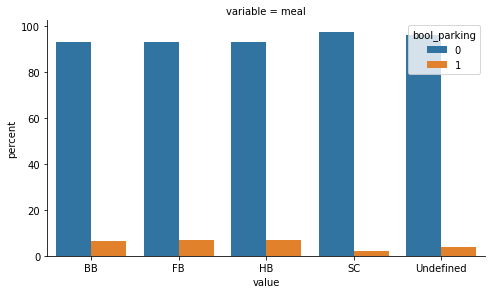
\includegraphics[width=0.9\textwidth]{img/TP2_KA_IB_files/TP2_KA_IB_80_0.png}

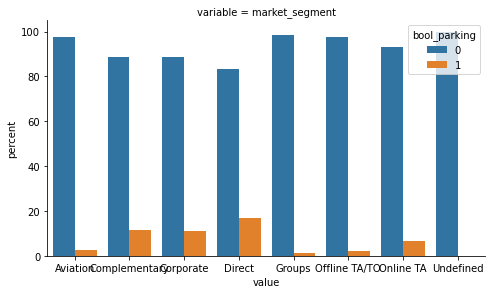
\includegraphics[width=0.9\textwidth]{img/TP2_KA_IB_files/TP2_KA_IB_80_1.png}

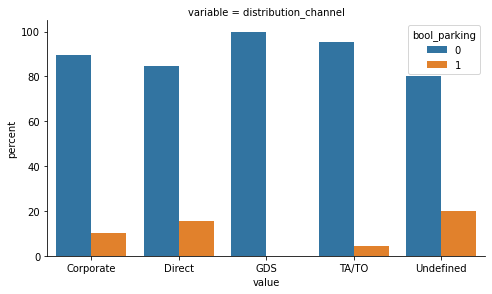
\includegraphics[width=0.9\textwidth]{img/TP2_KA_IB_files/TP2_KA_IB_80_2.png}

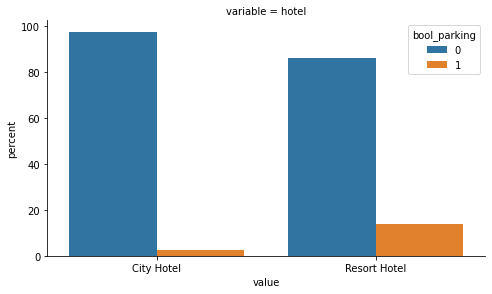
\includegraphics[width=0.9\textwidth]{img/TP2_KA_IB_files/TP2_KA_IB_80_3.png}

\end{col}

\begin{col}{0.5\textwidth}

\centering

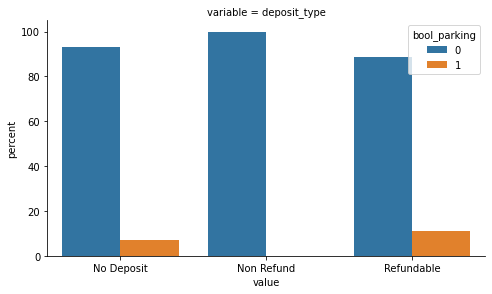
\includegraphics[width=0.9\textwidth]{img/TP2_KA_IB_files/TP2_KA_IB_80_5.png}

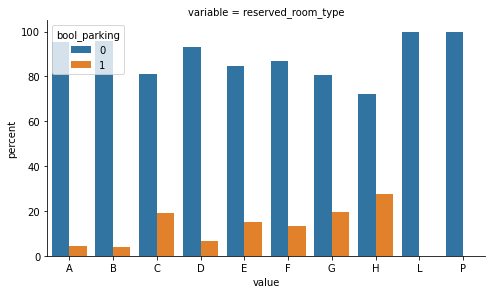
\includegraphics[width=0.9\textwidth]{img/TP2_KA_IB_files/TP2_KA_IB_80_4.png}

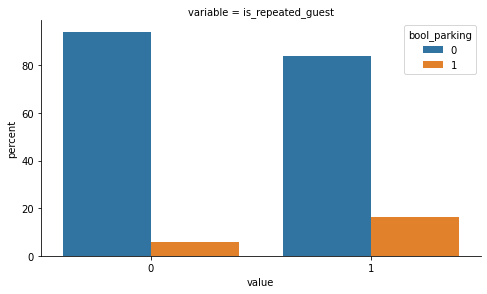
\includegraphics[width=0.9\textwidth]{img/TP2_KA_IB_files/TP2_KA_IB_80_7.png}

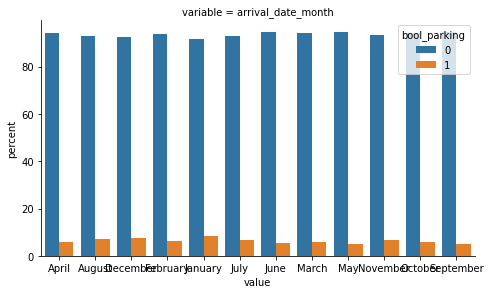
\includegraphics[width=0.9\textwidth]{img/TP2_KA_IB_files/TP2_KA_IB_80_8.png}

\end{col}

\begin{center}
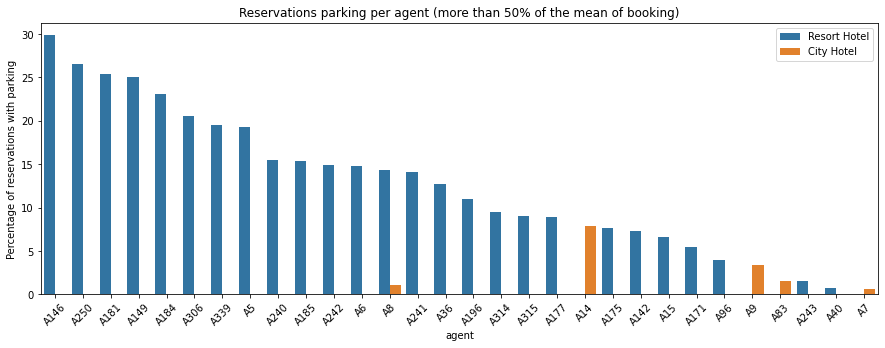
\includegraphics[width=0.8\textwidth]{img/TP2_KA_IB_files/TP2_KA_IB_81_0.png}
\end{center}

\newpage

\begin{center}
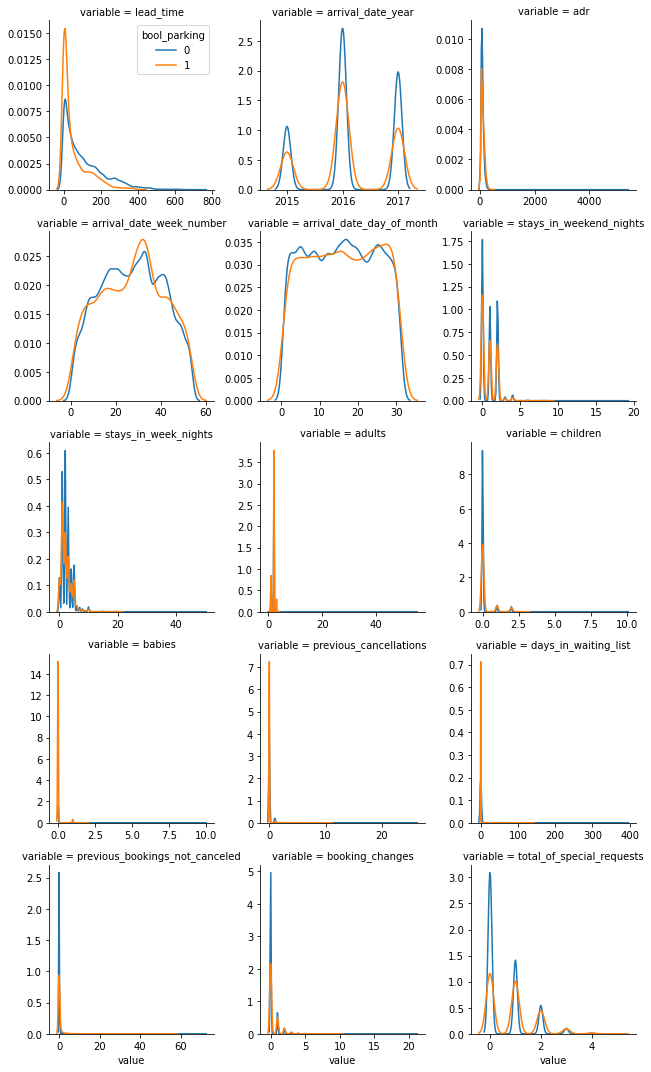
\includegraphics[width=0.9\textwidth]{img/TP2_KA_IB_files/TP2_KA_IB_82_1.png}
\end{center}

\newpage

\hypertarget{annexe:annexe5}{%
\section{Code of part III}\label{annexe:annexe5}}

\begin{Shaded}
\begin{Highlighting}[]
\CommentTok{#import packages for part III}
\ImportTok{from}\NormalTok{ sklearn.pipeline }\ImportTok{import}\NormalTok{ Pipeline}
\ImportTok{from}\NormalTok{ sklearn.compose }\ImportTok{import}\NormalTok{ ColumnTransformer}
\ImportTok{from}\NormalTok{ sklearn.preprocessing }\ImportTok{import}\NormalTok{ OneHotEncoder}
\ImportTok{from}\NormalTok{ sklearn.impute }\ImportTok{import}\NormalTok{ SimpleImputer}
\ImportTok{from}\NormalTok{ sklearn.linear_model }\ImportTok{import}\NormalTok{ LogisticRegression}
\ImportTok{from}\NormalTok{ sklearn.model_selection }\ImportTok{import}\NormalTok{ GridSearchCV}
\ImportTok{from}\NormalTok{ sklearn.preprocessing }\ImportTok{import}\NormalTok{ MinMaxScaler}
\ImportTok{from}\NormalTok{ sklearn.model_selection }\ImportTok{import}\NormalTok{ train_test_split}
\ImportTok{from}\NormalTok{ sklearn.utils }\ImportTok{import}\NormalTok{ shuffle}
\ImportTok{from}\NormalTok{ sklearn.svm }\ImportTok{import}\NormalTok{ LinearSVC}
\ImportTok{from}\NormalTok{ sklearn.preprocessing }\ImportTok{import}\NormalTok{ MinMaxScaler}
\ImportTok{from}\NormalTok{ sklearn.metrics }\ImportTok{import}\NormalTok{ accuracy_score}
\ImportTok{from}\NormalTok{ sklearn.metrics }\ImportTok{import}\NormalTok{ mean_squared_error}
\ImportTok{from}\NormalTok{ sklearn.metrics }\ImportTok{import}\NormalTok{ r2_score}
\end{Highlighting}
\end{Shaded}

\hypertarget{first-step-choose-the-relevant-features-and-build-the-dataset-1}{%
\subsection{FIRST STEP : choose the relevant features and build the dataset}\label{first-step-choose-the-relevant-features-and-build-the-dataset-1}}

\hypertarget{remove-features-with-too-many-missing-data}{%
\subsubsection{Remove features with too many missing data}\label{remove-features-with-too-many-missing-data}}

\begin{Shaded}
\begin{Highlighting}[]
\CommentTok{#Check Missing Data}
\NormalTok{plt.figure(figsize}\OperatorTok{=}\NormalTok{(}\DecValTok{10}\NormalTok{,}\DecValTok{4}\NormalTok{))}
\NormalTok{sns.heatmap(data.isna(),cbar}\OperatorTok{=}\VariableTok{False}\NormalTok{)}
\end{Highlighting}
\end{Shaded}

\hypertarget{creation-of-dataset}{%
\subsubsection{Creation of dataset}\label{creation-of-dataset}}

\begin{Shaded}
\begin{Highlighting}[]
\NormalTok{data2 }\OperatorTok{=}\NormalTok{ data.copy()}

\CommentTok{# New variable : boolean of value 1 if required_car_parking_spaces > 0}
\NormalTok{data2[}\StringTok{"bool_parking"}\NormalTok{] }\OperatorTok{=}\NormalTok{ data2[}\StringTok{"required_car_parking_spaces"}\NormalTok{] }\OperatorTok{>} \DecValTok{0} 
\NormalTok{data2[}\StringTok{"bool_parking"}\NormalTok{] }\OperatorTok{=}\NormalTok{ data2[}\StringTok{"bool_parking"}\NormalTok{].astype(}\BuiltInTok{int}\NormalTok{)}

\CommentTok{#We modify agent which is a strange variable (mix of numeric and categorical) by adding the prefix "A"}
\NormalTok{data2[}\StringTok{"agent"}\NormalTok{] }\OperatorTok{=}\NormalTok{ data2[}\StringTok{"agent"}\NormalTok{].}\BuiltInTok{map}\NormalTok{(}\KeywordTok{lambda}\NormalTok{ x:x }\ControlFlowTok{if}\NormalTok{ np.isnan(x) }\ControlFlowTok{else}\NormalTok{ (}\StringTok{"A"} \OperatorTok{+} \BuiltInTok{str}\NormalTok{(}\BuiltInTok{int}\NormalTok{(x))))}

\CommentTok{#We distinguish numerical and categorical features}
\NormalTok{numeric_features }\OperatorTok{=}\NormalTok{ [}\StringTok{"lead_time"}\NormalTok{, }\StringTok{"arrival_date_year"}\NormalTok{,}
                    \StringTok{"adr"}\NormalTok{,}
                    \StringTok{"arrival_date_week_number"}\NormalTok{,}
                    \StringTok{"arrival_date_day_of_month"}\NormalTok{, }\StringTok{"stays_in_weekend_nights"}\NormalTok{, }\StringTok{"stays_in_week_nights"}\NormalTok{, }
                    \StringTok{"adults"}\NormalTok{, }\StringTok{"children"}\NormalTok{,}
                    \StringTok{"babies"}\NormalTok{, }\StringTok{"previous_cancellations"}\NormalTok{, }
                    \StringTok{"days_in_waiting_list"}\NormalTok{, }\StringTok{"previous_bookings_not_canceled"}\NormalTok{, }\StringTok{"booking_changes"}\NormalTok{, }
                    \StringTok{"total_of_special_requests"}\NormalTok{]}
\NormalTok{categorical_features }\OperatorTok{=}\NormalTok{ [}\StringTok{"meal"}\NormalTok{, }\StringTok{"country"}\NormalTok{, }\StringTok{"market_segment"}\NormalTok{, }\StringTok{"distribution_channel"}\NormalTok{,}
                        \StringTok{"hotel"}\NormalTok{, }\StringTok{"reserved_room_type"}\NormalTok{, }\StringTok{"deposit_type"}\NormalTok{,}\StringTok{"agent"}\NormalTok{, }
                       \StringTok{"customer_type"}\NormalTok{,}\StringTok{"is_repeated_guest"}\NormalTok{,}\StringTok{"arrival_date_month"}\NormalTok{]                        }
\NormalTok{features }\OperatorTok{=}\NormalTok{ numeric_features }\OperatorTok{+}\NormalTok{ categorical_features}
\end{Highlighting}
\end{Shaded}

\hypertarget{second-step-exploratory-data-analysis-1}\NormalTok{matplotlib inline}
\CommentTok{#--------------------------------------------------------}
\CommentTok{############# categorical variables}
\NormalTok{variables }\OperatorTok{=}\NormalTok{ categorical_features.copy()}
\NormalTok{variables.append(}\StringTok{"bool_parking"}\NormalTok{)}
\NormalTok{variables.pop(}\DecValTok{7}\NormalTok{) }\CommentTok{#variable agent not very intersting to plot (to many of them)}
\NormalTok{variables.pop(}\DecValTok{1}\NormalTok{) }\CommentTok{#variable country not very intersting to plot (to many of them)}
\NormalTok{df }\OperatorTok{=}\NormalTok{ data2.}\BuiltInTok{filter}\NormalTok{(variables)}
\NormalTok{df }\OperatorTok{=}\NormalTok{ pd.melt(df, df.columns[}\OperatorTok{-}\DecValTok{1}\NormalTok{], df.columns[:}\OperatorTok{-}\DecValTok{1}\NormalTok{])}
\CommentTok{#df.head()}
\NormalTok{df }\OperatorTok{=}\NormalTok{ df.groupby([}\StringTok{'variable'}\NormalTok{,}\StringTok{'value'}\NormalTok{])[}\StringTok{'bool_parking'}\NormalTok{].value_counts(normalize}\OperatorTok{=}\VariableTok{True}\NormalTok{)}
\NormalTok{df }\OperatorTok{=}\NormalTok{ df.mul(}\DecValTok{100}\NormalTok{)}
\NormalTok{df }\OperatorTok{=}\NormalTok{ df.rename(}\StringTok{'percent'}\NormalTok{).reset_index()}

\ControlFlowTok{for}\NormalTok{ vExpl }\KeywordTok{in} \BuiltInTok{list}\NormalTok{(variables):}
    \ControlFlowTok{if}\NormalTok{ vExpl }\OperatorTok{!=} \StringTok{'bool_parking'}\NormalTok{:}
\NormalTok{        data_graph }\OperatorTok{=}\NormalTok{ df[(df[}\StringTok{'variable'}\NormalTok{] }\OperatorTok{==}\NormalTok{ vExpl)]}
\NormalTok{        g }\OperatorTok{=}\NormalTok{ sns.catplot(x}\OperatorTok{=}\StringTok{"value"}\NormalTok{, y}\OperatorTok{=}\StringTok{"percent"}\NormalTok{, hue}\OperatorTok{=}\StringTok{"bool_parking"}\NormalTok{, col}\OperatorTok{=}\StringTok{"variable"}\NormalTok{, data}\OperatorTok{=}\NormalTok{data_graph,}
\NormalTok{               col_wrap}\OperatorTok{=}\DecValTok{3}\NormalTok{, kind}\OperatorTok{=}\StringTok{"bar"}\NormalTok{, sharex}\OperatorTok{=}\VariableTok{False}\NormalTok{, sharey}\OperatorTok{=}\VariableTok{True}\NormalTok{,legend_out}\OperatorTok{=}\VariableTok{False}\NormalTok{, height}\OperatorTok{=}\DecValTok{4}\NormalTok{,aspect}\OperatorTok{=}\FloatTok{1.6}\NormalTok{)}
\end{Highlighting}
\end{Shaded}

\begin{Shaded}
\begin{Highlighting}[]
\CommentTok{#---------------------------------------------------------------------------------------------}
\CommentTok{#Agent : Percentage of reservations with parking for agent with more than 50% mean of bookings}
\CommentTok{#        (exclude percentage with few reservations)}
\CommentTok{#---------------------------------------------------------------------------------------------}
\NormalTok{n_reserv_byagent_H1 }\OperatorTok{=}\NormalTok{ data2.loc[}
\NormalTok{    (data[}\StringTok{"hotel"}\NormalTok{] }\OperatorTok{==} \StringTok{"Resort Hotel"}\NormalTok{)].groupby(}\StringTok{"agent"}\NormalTok{)[}\StringTok{"hotel"}\NormalTok{].count()}
\NormalTok{n_bparking_byagent_H1 }\OperatorTok{=}\NormalTok{ data2.loc[}
\NormalTok{    (data2[}\StringTok{"hotel"}\NormalTok{] }\OperatorTok{==} \StringTok{"Resort Hotel"}\NormalTok{)].groupby(}\StringTok{"agent"}\NormalTok{)[}\StringTok{"bool_parking"}\NormalTok{].}\BuiltInTok{sum}\NormalTok{()}
\NormalTok{data_agent_visualH1 }\OperatorTok{=}\NormalTok{ pd.DataFrame(\{}\StringTok{"hotel"}\NormalTok{: }\StringTok{"Resort Hotel"}\NormalTok{,}
                                \StringTok{"agent"}\NormalTok{: }\BuiltInTok{list}\NormalTok{(n_reserv_byagent_H1.index),}
                                \StringTok{"n_booking"}\NormalTok{: }\BuiltInTok{list}\NormalTok{(n_reserv_byagent_H1.values),}
                                \StringTok{"n_bool_parking"}\NormalTok{: }\BuiltInTok{list}\NormalTok{(n_bparking_byagent_H1.values)\})}
\NormalTok{data_agent_visualH1.sort_values(by}\OperatorTok{=}\NormalTok{[}\StringTok{'n_bool_parking'}\NormalTok{], ascending}\OperatorTok{=}\VariableTok{False}\NormalTok{)}
\NormalTok{n_reserv_byagent_H2 }\OperatorTok{=}\NormalTok{ data2.loc[}
\NormalTok{    (data[}\StringTok{"hotel"}\NormalTok{] }\OperatorTok{==} \StringTok{"City Hotel"}\NormalTok{)].groupby(}\StringTok{"agent"}\NormalTok{)[}\StringTok{"hotel"}\NormalTok{].count()}
\NormalTok{n_bparking_byagent_H2 }\OperatorTok{=}\NormalTok{ data2.loc[}
\NormalTok{    (data2[}\StringTok{"hotel"}\NormalTok{] }\OperatorTok{==} \StringTok{"City Hotel"}\NormalTok{)].groupby(}\StringTok{"agent"}\NormalTok{)[}\StringTok{"bool_parking"}\NormalTok{].}\BuiltInTok{sum}\NormalTok{()}
\NormalTok{data_agent_visualH2 }\OperatorTok{=}\NormalTok{ pd.DataFrame(\{}\StringTok{"hotel"}\NormalTok{: }\StringTok{"City Hotel"}\NormalTok{,}
                                \StringTok{"agent"}\NormalTok{: }\BuiltInTok{list}\NormalTok{(n_reserv_byagent_H2.index),}
                                \StringTok{"n_booking"}\NormalTok{: }\BuiltInTok{list}\NormalTok{(n_reserv_byagent_H2.values),}
                                \StringTok{"n_bool_parking"}\NormalTok{: }\BuiltInTok{list}\NormalTok{(n_bparking_byagent_H2.values)\})}
\NormalTok{data_agent_visualH2.sort_values(by}\OperatorTok{=}\NormalTok{[}\StringTok{'n_bool_parking'}\NormalTok{], ascending}\OperatorTok{=}\VariableTok{False}\NormalTok{)}
\NormalTok{data_agent_visual }\OperatorTok{=}\NormalTok{ pd.concat([data_agent_visualH1, data_agent_visualH2], ignore_index}\OperatorTok{=}\VariableTok{True}\NormalTok{)}
\NormalTok{data_agent_visual[}\StringTok{"percent_bParking"}\NormalTok{] }\OperatorTok{=}\NormalTok{ data_agent_visual[}
    \StringTok{"n_bool_parking"}\NormalTok{] }\OperatorTok{/}\NormalTok{ data_agent_visual[}\StringTok{"n_booking"}\NormalTok{] }\OperatorTok{*} \DecValTok{100} \CommentTok{# percent of parking}
\NormalTok{data_agent_visual }\OperatorTok{=}\NormalTok{ data_agent_visual.sort_values(by}\OperatorTok{=}\NormalTok{[}\StringTok{'percent_bParking'}\NormalTok{], ascending}\OperatorTok{=}\VariableTok{False}\NormalTok{)}
\NormalTok{plt.figure(figsize}\OperatorTok{=}\NormalTok{(}\DecValTok{15}\NormalTok{, }\DecValTok{5}\NormalTok{))}
\NormalTok{sns.barplot(x }\OperatorTok{=} \StringTok{"agent"}\NormalTok{, y }\OperatorTok{=} \StringTok{"percent_bParking"}\NormalTok{ , hue}\OperatorTok{=}\StringTok{"hotel"}\NormalTok{,}
\NormalTok{            hue_order }\OperatorTok{=}\NormalTok{ [}\StringTok{"Resort Hotel"}\NormalTok{, }\StringTok{"City Hotel"}\NormalTok{], }
\NormalTok{            data}\OperatorTok{=}\NormalTok{data_agent_visual[}
\NormalTok{                data_agent_visual[}\StringTok{"n_bool_parking"}\NormalTok{]}\OperatorTok{>}\FloatTok{0.5}\OperatorTok{*}\NormalTok{np.mean(data_agent_visual[}\StringTok{"n_bool_parking"}\NormalTok{])])}
\NormalTok{plt.title(}\StringTok{"Reservations parking per agent (more than 50}\SpecialCharTok{% o}\StringTok{f the mean of booking)"}\NormalTok{)}
\NormalTok{plt.xticks(rotation}\OperatorTok{=}\DecValTok{45}\NormalTok{)}
\NormalTok{plt.ylabel(}\StringTok{"Percentage of reservations with parking"}\NormalTok{)}
\NormalTok{plt.legend()}
\NormalTok{plt.show()}
\end{Highlighting}
\end{Shaded}

\begin{Shaded}
\begin{Highlighting}[]
\CommentTok{############# numeric variables}
\NormalTok{sns.distributions._has_statsmodels }\OperatorTok{=} \VariableTok{False}
\NormalTok{variables }\OperatorTok{=}\NormalTok{ numeric_features.copy()}
\NormalTok{variables.append(}\StringTok{"bool_parking"}\NormalTok{)}
\NormalTok{df }\OperatorTok{=}\NormalTok{ data2.}\BuiltInTok{filter}\NormalTok{(variables)}
\NormalTok{df }\OperatorTok{=}\NormalTok{ pd.melt(df, df.columns[}\OperatorTok{-}\DecValTok{1}\NormalTok{], df.columns[:}\OperatorTok{-}\DecValTok{1}\NormalTok{])}
\NormalTok{g }\OperatorTok{=}\NormalTok{ sns.FacetGrid(df, col}\OperatorTok{=}\StringTok{"variable"}\NormalTok{, hue}\OperatorTok{=}\StringTok{"bool_parking"}\NormalTok{,}
\NormalTok{                  col_wrap}\OperatorTok{=}\DecValTok{3}\NormalTok{,sharex}\OperatorTok{=}\VariableTok{False}\NormalTok{, sharey}\OperatorTok{=}\VariableTok{False}\NormalTok{,legend_out}\OperatorTok{=}\VariableTok{False}\NormalTok{)}
\NormalTok{g.}\BuiltInTok{map}\NormalTok{(sns.kdeplot, }\StringTok{"value"}\NormalTok{) }\CommentTok{#, shade=True}
\NormalTok{g.add_legend()}
\end{Highlighting}
\end{Shaded}

\hypertarget{third-step-modelisation-1}{%
\subsection{THIRD STEP : Modelisation}\label{third-step-modelisation-1}}

\hypertarget{models-including-all-the-variables-1}{%
\subsubsection{Models including all the variables}\label{models-including-all-the-variables-1}}

\textbf{Preparing the test and training sets}

\begin{Shaded}
\begin{Highlighting}[]
\CommentTok{#--------------------------------------------------------------------------------}
\CommentTok{# Feature Engineering : Process of converting raw data into a structured format }
\CommentTok{# Making the data ready to use for model training (transformers)}
\CommentTok{# Creating the test and training sets}
\CommentTok{#--------------------------------------------------------------------------------}
\NormalTok{numeric_transformer }\OperatorTok{=}\NormalTok{ Pipeline(steps}\OperatorTok{=}\NormalTok{[}
\NormalTok{                                    (}\StringTok{"imputer"}\NormalTok{, SimpleImputer(strategy}\OperatorTok{=}\StringTok{"constant"}\NormalTok{, fill_value}\OperatorTok{=}\DecValTok{0}\NormalTok{)),}
\NormalTok{                                    (}\StringTok{"scaler"}\NormalTok{, MinMaxScaler())]) }
\NormalTok{categorical_transformer }\OperatorTok{=}\NormalTok{ Pipeline(steps}\OperatorTok{=}\NormalTok{[}
\NormalTok{                                    (}\StringTok{"imputer"}\NormalTok{, SimpleImputer(strategy}\OperatorTok{=}\StringTok{"constant"}\NormalTok{,}
\NormalTok{                                    fill_value}\OperatorTok{=}\StringTok{"Not defined"}\NormalTok{)),}
\NormalTok{                                    (}\StringTok{"onehot"}\NormalTok{, OneHotEncoder(handle_unknown}\OperatorTok{=}\StringTok{'ignore'}\NormalTok{))]) }\CommentTok{#}
\NormalTok{preproc }\OperatorTok{=}\NormalTok{ ColumnTransformer(transformers}\OperatorTok{=}\NormalTok{[(}\StringTok{"num"}\NormalTok{, numeric_transformer, numeric_features),}
\NormalTok{                                          (}\StringTok{"cat"}\NormalTok{, categorical_transformer, categorical_features)])}

\NormalTok{X }\OperatorTok{=}\NormalTok{ data2.drop([}\StringTok{"is_canceled"}\NormalTok{,}\StringTok{"assigned_room_type"}\NormalTok{,}\StringTok{"reservation_status"}\NormalTok{,}
\StringTok{"reservation_status_date"}\NormalTok{,}\StringTok{"company"}\NormalTok{],}
\NormalTok{              axis}\OperatorTok{=}\DecValTok{1}\NormalTok{)[features]}
\NormalTok{y }\OperatorTok{=}\NormalTok{ data2[}\StringTok{"bool_parking"}\NormalTok{]}

\NormalTok{X, y }\OperatorTok{=}\NormalTok{ shuffle(X,y)}
\NormalTok{X_train, X_test, y_train, y_test }\OperatorTok{=}\NormalTok{ train_test_split(X, y)}

\NormalTok{X_preproc }\OperatorTok{=}\NormalTok{ preproc.fit_transform(X)}
\NormalTok{X_train_preproc, X_test_preproc, y_train_preproc, y_test_preproc }\OperatorTok{=}\NormalTok{ train_test_split(X_preproc, y)}
\end{Highlighting}
\end{Shaded}

\textbf{Running the models using Cross-validation}

\begin{Shaded}
\begin{Highlighting}[]
\NormalTok{models }\OperatorTok{=}\NormalTok{ [(}\StringTok{"logreg"}\NormalTok{, LogisticRegression(max_iter}\OperatorTok{=}\DecValTok{700}\NormalTok{)),}
\NormalTok{          (}\StringTok{"svc"}\NormalTok{, LinearSVC(max_iter}\OperatorTok{=}\DecValTok{800}\NormalTok{))]}
\NormalTok{grids }\OperatorTok{=}\NormalTok{ \{}\StringTok{"logreg"}\NormalTok{ : \{}\StringTok{'logreg__C'}\NormalTok{: np.logspace(}\OperatorTok{-}\DecValTok{2}\NormalTok{, }\DecValTok{2}\NormalTok{, }\DecValTok{5}\NormalTok{, base}\OperatorTok{=}\DecValTok{2}\NormalTok{)\},}
         \StringTok{"svc"}\NormalTok{ : \{}\StringTok{'svc__C'}\NormalTok{: np.logspace(}\OperatorTok{-}\DecValTok{2}\NormalTok{, }\DecValTok{2}\NormalTok{, }\DecValTok{5}\NormalTok{, base}\OperatorTok{=}\DecValTok{2}\NormalTok{)\}\}}
\NormalTok{X_train, X_test, y_train, y_test }\OperatorTok{=}\NormalTok{ train_test_split(X, y)}

\ControlFlowTok{for}\NormalTok{ name, model }\KeywordTok{in}\NormalTok{ models:}
\NormalTok{    pipe }\OperatorTok{=}\NormalTok{ Pipeline(steps}\OperatorTok{=}\NormalTok{[(}\StringTok{'preprocessor'}\NormalTok{, preproc), (name, model)])}
\NormalTok{    clf }\OperatorTok{=}\NormalTok{ GridSearchCV(pipe, grids[name], cv}\OperatorTok{=}\DecValTok{3}\NormalTok{)}
\NormalTok{    clf.fit(X_train, y_train)}
    \BuiltInTok{print}\NormalTok{(}\StringTok{'Results for }\SpecialCharTok{\{\}}\StringTok{'}\NormalTok{.}\BuiltInTok{format}\NormalTok{(name))}
    \BuiltInTok{print}\NormalTok{(}\StringTok{'Returned hyperparameter: }\SpecialCharTok{\{\}}\StringTok{'}\NormalTok{.}\BuiltInTok{format}\NormalTok{(clf.best_params_))}
    \BuiltInTok{print}\NormalTok{(}\StringTok{'Best classification accuracy in train is: }\SpecialCharTok{\{\}}\StringTok{'}\NormalTok{.}\BuiltInTok{format}\NormalTok{(clf.best_score_))}
    \BuiltInTok{print}\NormalTok{(}\StringTok{'Classification accuracy on test is: }\SpecialCharTok{\{\}}\StringTok{'}\NormalTok{.}\BuiltInTok{format}\NormalTok{(clf.score(X_test, y_test)))    }
\NormalTok{    display(pd.DataFrame(clf.cv_results_)[[}\StringTok{'params'}\NormalTok{,}\StringTok{'mean_test_score'}\NormalTok{, }\StringTok{'std_test_score'}\NormalTok{,}
                                           \StringTok{'rank_test_score'}\NormalTok{]])}
\end{Highlighting}
\end{Shaded}

\textbf{Running the models with the best parameters and evaluating with different scores}

\begin{Shaded}
\begin{Highlighting}[]
\NormalTok{logreg }\OperatorTok{=}\NormalTok{ LogisticRegression(max_iter}\OperatorTok{=}\DecValTok{700}\NormalTok{, C}\OperatorTok{=}\FloatTok{0.25}\NormalTok{) }\CommentTok{#best parameter logreg : C=0.25}
\NormalTok{logreg.fit(X_train_preproc,y_train_preproc)}
\NormalTok{y_pred }\OperatorTok{=}\NormalTok{ logreg.predict(X_test_preproc)}
\BuiltInTok{print}\NormalTok{(}\StringTok{"MSE logreg: "}\NormalTok{, mean_squared_error(y_test_preproc, y_pred, squared}\OperatorTok{=}\VariableTok{False}\NormalTok{))}
\BuiltInTok{print}\NormalTok{(}\StringTok{"R2 logreg: "}\NormalTok{, r2_score(y_test, y_pred))}
\BuiltInTok{print}\NormalTok{(}\StringTok{"accuracy logreg : "}\NormalTok{, accuracy_score(y_test_preproc, y_pred)) }\CommentTok{#OK because Y_pred is binary}

\BuiltInTok{print}\NormalTok{(}\StringTok{"}\CharTok{\textbackslash{}n}\StringTok{"}\NormalTok{)}

\NormalTok{svc }\OperatorTok{=}\NormalTok{ LinearSVC(max_iter}\OperatorTok{=}\DecValTok{800}\NormalTok{, C}\OperatorTok{=}\FloatTok{0.25}\NormalTok{) }\CommentTok{#best parameter svc : C=0.25}
\NormalTok{svc.fit(X_train_preproc,y_train_preproc)}
\NormalTok{y_pred }\OperatorTok{=}\NormalTok{ svc.predict(X_test_preproc)}
\BuiltInTok{print}\NormalTok{(}\StringTok{"MSE svc: "}\NormalTok{, mean_squared_error(y_test_preproc, y_pred, squared}\OperatorTok{=}\VariableTok{False}\NormalTok{))}
\BuiltInTok{print}\NormalTok{(}\StringTok{"R2 svc: "}\NormalTok{, r2_score(y_test_preproc, y_pred))}
\BuiltInTok{print}\NormalTok{(}\StringTok{"accuracy svc : "}\NormalTok{, accuracy_score(y_test_preproc, y_pred)) }\CommentTok{#OK because Y_pred is binary}
\end{Highlighting}
\end{Shaded}

\hypertarget{models-with-best-predictive-features-chosen-manually-1}{%
\subsubsection{Models with best predictive features chosen MANUALLY}\label{models-with-best-predictive-features-chosen-manually-1}}

\textbf{Preparing the test and training sets}

\begin{Shaded}
\begin{Highlighting}[]
\NormalTok{dataHW }\OperatorTok{=}\NormalTok{ data2.copy()}

\CommentTok{#--------------------------------------------------------------------------------}
\CommentTok{# Feature Selection : Picking up the most predictive features }
\CommentTok{#--------------------------------------------------------------------------------}
\NormalTok{numeric_features }\OperatorTok{=}\NormalTok{ [}\StringTok{"arrival_date_week_number"}\NormalTok{,}\StringTok{"lead_time"}\NormalTok{, }\StringTok{"adr"}\NormalTok{,}\StringTok{"children"}\NormalTok{]}
\NormalTok{categorical_features }\OperatorTok{=}\NormalTok{ [}\StringTok{"customer_type"}\NormalTok{,}\StringTok{"hotel"}\NormalTok{, }\StringTok{"market_segment"}\NormalTok{, }\StringTok{"reserved_room_type"}\NormalTok{]                       }
\NormalTok{features }\OperatorTok{=}\NormalTok{ numeric_features }\OperatorTok{+}\NormalTok{ categorical_features}

\CommentTok{#--------------------------------------------------------------------------------}
\CommentTok{# Feature Engineering : Process of converting raw data into a structured format }
\CommentTok{# Making the data ready to use for model training (transformers)}
\CommentTok{# Creating the test and training sets}
\CommentTok{#--------------------------------------------------------------------------------}
\NormalTok{numeric_transformer }\OperatorTok{=}\NormalTok{ Pipeline(steps}\OperatorTok{=}\NormalTok{[}
\NormalTok{                                    (}\StringTok{"imputer"}\NormalTok{, SimpleImputer(strategy}\OperatorTok{=}\StringTok{"constant"}\NormalTok{, fill_value}\OperatorTok{=}\DecValTok{0}\NormalTok{)),}
\NormalTok{                                    (}\StringTok{"scaler"}\NormalTok{, MinMaxScaler())]) }
\NormalTok{categorical_transformer }\OperatorTok{=}\NormalTok{ Pipeline(steps}\OperatorTok{=}\NormalTok{[}
\NormalTok{                                    (}\StringTok{"imputer"}\NormalTok{, SimpleImputer(strategy}\OperatorTok{=}\StringTok{"constant"}\NormalTok{,}
\NormalTok{                                    fill_value}\OperatorTok{=}\StringTok{"Not defined"}\NormalTok{)),}
\NormalTok{                                    (}\StringTok{"onehot"}\NormalTok{, OneHotEncoder(handle_unknown}\OperatorTok{=}\StringTok{'ignore'}\NormalTok{))])}
\NormalTok{preproc }\OperatorTok{=}\NormalTok{ ColumnTransformer(transformers}\OperatorTok{=}\NormalTok{[(}\StringTok{"num"}\NormalTok{, numeric_transformer, numeric_features),}
\NormalTok{                                          (}\StringTok{"cat"}\NormalTok{, categorical_transformer, categorical_features)])}

\NormalTok{X }\OperatorTok{=}\NormalTok{ dataHW[features]}
\NormalTok{y }\OperatorTok{=}\NormalTok{ dataHW[}\StringTok{"bool_parking"}\NormalTok{]}

\NormalTok{X, y }\OperatorTok{=}\NormalTok{ shuffle(X,y)}
\NormalTok{X_train, X_test, y_train, y_test }\OperatorTok{=}\NormalTok{ train_test_split(X, y)}

\NormalTok{X_preproc }\OperatorTok{=}\NormalTok{ preproc.fit_transform(X)}
\NormalTok{X_train_preproc, X_test_preproc, y_train_preproc, y_test_preproc }\OperatorTok{=}\NormalTok{ train_test_split(X_preproc, y)}
\end{Highlighting}
\end{Shaded}

\textbf{Running the models using Cross-validation}

\begin{Shaded}
\begin{Highlighting}[]
\NormalTok{models }\OperatorTok{=}\NormalTok{ [(}\StringTok{"logreg"}\NormalTok{, LogisticRegression(max_iter}\OperatorTok{=}\DecValTok{700}\NormalTok{)),}
\NormalTok{          (}\StringTok{"svc"}\NormalTok{, LinearSVC(max_iter}\OperatorTok{=}\DecValTok{800}\NormalTok{))]}
\NormalTok{grids }\OperatorTok{=}\NormalTok{ \{}\StringTok{"logreg"}\NormalTok{ : \{}\StringTok{'logreg__C'}\NormalTok{: np.logspace(}\OperatorTok{-}\DecValTok{2}\NormalTok{, }\DecValTok{2}\NormalTok{, }\DecValTok{5}\NormalTok{, base}\OperatorTok{=}\DecValTok{2}\NormalTok{)\},}
         \StringTok{"svc"}\NormalTok{ : \{}\StringTok{'svc__C'}\NormalTok{: np.logspace(}\OperatorTok{-}\DecValTok{2}\NormalTok{, }\DecValTok{2}\NormalTok{, }\DecValTok{5}\NormalTok{, base}\OperatorTok{=}\DecValTok{2}\NormalTok{)\}\}}
\ControlFlowTok{for}\NormalTok{ name, model }\KeywordTok{in}\NormalTok{ models:}
\NormalTok{    pipe }\OperatorTok{=}\NormalTok{ Pipeline(steps}\OperatorTok{=}\NormalTok{[(}\StringTok{'preprocessor'}\NormalTok{, preproc), (name, model)])}
\NormalTok{    clf }\OperatorTok{=}\NormalTok{ GridSearchCV(pipe, grids[name], cv}\OperatorTok{=}\DecValTok{3}\NormalTok{)}
\NormalTok{    clf.fit(X_train, y_train)}
    \BuiltInTok{print}\NormalTok{(}\StringTok{'Results for }\SpecialCharTok{\{\}}\StringTok{'}\NormalTok{.}\BuiltInTok{format}\NormalTok{(name))}
    \BuiltInTok{print}\NormalTok{(}\StringTok{'Returned hyperparameter: }\SpecialCharTok{\{\}}\StringTok{'}\NormalTok{.}\BuiltInTok{format}\NormalTok{(clf.best_params_))}
    \BuiltInTok{print}\NormalTok{(}\StringTok{'Best classification accuracy in train is: }\SpecialCharTok{\{\}}\StringTok{'}\NormalTok{.}\BuiltInTok{format}\NormalTok{(clf.best_score_))}
    \BuiltInTok{print}\NormalTok{(}\StringTok{'Classification accuracy on test is: }\SpecialCharTok{\{\}}\StringTok{'}\NormalTok{.}\BuiltInTok{format}\NormalTok{(clf.score(X_test, y_test)))    }
\NormalTok{    display(pd.DataFrame(clf.cv_results_)[[}\StringTok{'params'}\NormalTok{,}\StringTok{'mean_test_score'}\NormalTok{, }\StringTok{'std_test_score'}\NormalTok{,}
                                           \StringTok{'rank_test_score'}\NormalTok{]])}
\end{Highlighting}
\end{Shaded}

\textbf{Running the models with the best parameters and evaluating with different scores}

\begin{Shaded}
\begin{Highlighting}[]
\NormalTok{logreg }\OperatorTok{=}\NormalTok{ LogisticRegression(max_iter}\OperatorTok{=}\DecValTok{700}\NormalTok{, C}\OperatorTok{=}\FloatTok{0.25}\NormalTok{) }\CommentTok{#best parameter logreg : C=0.25}
\NormalTok{logreg.fit(X_train_preproc,y_train_preproc)}
\NormalTok{y_pred }\OperatorTok{=}\NormalTok{ logreg.predict(X_test_preproc)}
\BuiltInTok{print}\NormalTok{(}\StringTok{"MSE logreg: "}\NormalTok{, mean_squared_error(y_test_preproc, y_pred, squared}\OperatorTok{=}\VariableTok{False}\NormalTok{))}
\BuiltInTok{print}\NormalTok{(}\StringTok{"R2 logreg: "}\NormalTok{, r2_score(y_test, y_pred))}
\BuiltInTok{print}\NormalTok{(}\StringTok{"accuracy logreg : "}\NormalTok{, accuracy_score(y_test_preproc, y_pred)) }\CommentTok{#OK because Y_pred is binary}

\BuiltInTok{print}\NormalTok{(}\StringTok{"}\CharTok{\textbackslash{}n}\StringTok{"}\NormalTok{)}

\NormalTok{svc }\OperatorTok{=}\NormalTok{ LinearSVC(max_iter}\OperatorTok{=}\DecValTok{800}\NormalTok{, C}\OperatorTok{=}\FloatTok{0.25}\NormalTok{) }\CommentTok{#best parameter svc : C=0.25}
\NormalTok{svc.fit(X_train_preproc,y_train_preproc)}
\NormalTok{y_pred }\OperatorTok{=}\NormalTok{ svc.predict(X_test_preproc)}
\BuiltInTok{print}\NormalTok{(}\StringTok{"MSE svc: "}\NormalTok{, mean_squared_error(y_test_preproc, y_pred, squared}\OperatorTok{=}\VariableTok{False}\NormalTok{))}
\BuiltInTok{print}\NormalTok{(}\StringTok{"R2 svc: "}\NormalTok{, r2_score(y_test_preproc, y_pred))}
\BuiltInTok{print}\NormalTok{(}\StringTok{"accuracy svc : "}\NormalTok{, accuracy_score(y_test_preproc, y_pred)) }\CommentTok{#OK because Y_pred is binary}
\end{Highlighting}
\end{Shaded}

\hypertarget{models-with-best-predictive-features-chosen-with-regularized-regressions-1}{%
\subsubsection{Models with best predictive features chosen with REGULARIZED REGRESSIONS}\label{models-with-best-predictive-features-chosen-with-regularized-regressions-1}}

\textbf{Preparing the test and training sets}

\begin{Shaded}
\begin{Highlighting}[]
\CommentTok{#--------------------------------------------------------------------------------}
\CommentTok{# Feature Selection : Picking up the most predictive features }
\CommentTok{#--------------------------------------------------------------------------------}
\CommentTok{#We distinguish numerical and categorical features}
\NormalTok{numeric_features }\OperatorTok{=}\NormalTok{ [}\StringTok{"lead_time"}\NormalTok{, }\StringTok{"arrival_date_year"}\NormalTok{,}
                    \StringTok{"adr"}\NormalTok{,}
                    \StringTok{"arrival_date_week_number"}\NormalTok{,}
                    \StringTok{"arrival_date_day_of_month"}\NormalTok{, }\StringTok{"stays_in_weekend_nights"}\NormalTok{, }\StringTok{"stays_in_week_nights"}\NormalTok{, }
                    \StringTok{"adults"}\NormalTok{, }\StringTok{"children"}\NormalTok{,}
                    \StringTok{"babies"}\NormalTok{, }\StringTok{"previous_cancellations"}\NormalTok{, }
                    \StringTok{"days_in_waiting_list"}\NormalTok{, }\StringTok{"previous_bookings_not_canceled"}\NormalTok{, }\StringTok{"booking_changes"}\NormalTok{, }
                    \StringTok{"total_of_special_requests"}\NormalTok{]}
\NormalTok{categorical_features }\OperatorTok{=}\NormalTok{ [}\StringTok{"meal"}\NormalTok{, }\StringTok{"country"}\NormalTok{, }\StringTok{"market_segment"}\NormalTok{, }\StringTok{"distribution_channel"}\NormalTok{,}
                        \StringTok{"hotel"}\NormalTok{, }\StringTok{"reserved_room_type"}\NormalTok{, }\StringTok{"deposit_type"}\NormalTok{,}\StringTok{"agent"}\NormalTok{, }
                       \StringTok{"customer_type"}\NormalTok{,}\StringTok{"is_repeated_guest"}\NormalTok{,}\StringTok{"arrival_date_month"}\NormalTok{]                        }
\NormalTok{features }\OperatorTok{=}\NormalTok{ numeric_features }\OperatorTok{+}\NormalTok{ categorical_features}

\CommentTok{#--------------------------------------------------------------------------------}
\CommentTok{# Feature Engineering : Process of converting raw data into a structured format }
\CommentTok{# Making the data ready to use for model training (transformers)}
\CommentTok{# Creating the test and training sets}
\CommentTok{#--------------------------------------------------------------------------------}

\NormalTok{numeric_transformer }\OperatorTok{=}\NormalTok{ Pipeline(steps}\OperatorTok{=}\NormalTok{[}
\NormalTok{                                    (}\StringTok{"imputer"}\NormalTok{, SimpleImputer(strategy}\OperatorTok{=}\StringTok{"constant"}\NormalTok{, fill_value}\OperatorTok{=}\DecValTok{0}\NormalTok{)),}
\NormalTok{                                    (}\StringTok{"scaler"}\NormalTok{, MinMaxScaler())]) }
\NormalTok{categorical_transformer }\OperatorTok{=}\NormalTok{ Pipeline(steps}\OperatorTok{=}\NormalTok{[}
\NormalTok{                                    (}\StringTok{"imputer"}\NormalTok{, SimpleImputer(strategy}\OperatorTok{=}\StringTok{"constant"}\NormalTok{,}
\NormalTok{                                    fill_value}\OperatorTok{=}\StringTok{"Not defined"}\NormalTok{)),}
\NormalTok{                                    (}\StringTok{"onehot"}\NormalTok{, OneHotEncoder(handle_unknown}\OperatorTok{=}\StringTok{'ignore'}\NormalTok{))]) }\CommentTok{#}
\NormalTok{preproc }\OperatorTok{=}\NormalTok{ ColumnTransformer(transformers}\OperatorTok{=}\NormalTok{[(}\StringTok{"num"}\NormalTok{, numeric_transformer, numeric_features),}
\NormalTok{                                          (}\StringTok{"cat"}\NormalTok{, categorical_transformer, categorical_features)])}

\NormalTok{X }\OperatorTok{=}\NormalTok{ data2.drop([}\StringTok{"is_canceled"}\NormalTok{,}\StringTok{"assigned_room_type"}\NormalTok{,}\StringTok{"reservation_status"}\NormalTok{,}
\StringTok{"reservation_status_date"}\NormalTok{, }\StringTok{"company"}\NormalTok{],}
\NormalTok{              axis}\OperatorTok{=}\DecValTok{1}\NormalTok{)[features]}
\NormalTok{y }\OperatorTok{=}\NormalTok{ data2[}\StringTok{"bool_parking"}\NormalTok{]}

\NormalTok{X, y }\OperatorTok{=}\NormalTok{ shuffle(X,y)}
\NormalTok{X_train, X_test, y_train, y_test }\OperatorTok{=}\NormalTok{ train_test_split(X, y)}

\NormalTok{X_preproc }\OperatorTok{=}\NormalTok{ preproc.fit_transform(X)}
\NormalTok{X_train_preproc, X_test_preproc, y_train_preproc, y_test_preproc }\OperatorTok{=}\NormalTok{ train_test_split(X_preproc, y)}
\end{Highlighting}
\end{Shaded}

\textbf{Running the model using Cross-validation}

\begin{Shaded}
\begin{Highlighting}[]
\CommentTok{#lasso path }
\ImportTok{from}\NormalTok{ sklearn.linear_model }\ImportTok{import}\NormalTok{ lasso_path}
\NormalTok{my_alphas }\OperatorTok{=}\NormalTok{ np.array([}\FloatTok{0.001}\NormalTok{,}\FloatTok{0.01}\NormalTok{,}\FloatTok{0.02}\NormalTok{,}\FloatTok{0.025}\NormalTok{,}\FloatTok{0.05}\NormalTok{,}\FloatTok{0.1}\NormalTok{,}\FloatTok{0.25}\NormalTok{,}\FloatTok{0.5}\NormalTok{,}\FloatTok{0.8}\NormalTok{,}\FloatTok{1.0}\NormalTok{])}
\NormalTok{alpha_for_path, coefs_lasso, _ }\OperatorTok{=}\NormalTok{ lasso_path(X_train_preproc,y,alphas}\OperatorTok{=}\NormalTok{my_alphas)}
\NormalTok{nb_coeff }\OperatorTok{=}\NormalTok{ coefs_lasso.shape[}\DecValTok{0}\NormalTok{] }\CommentTok{#578}
\NormalTok{nb_alpha }\OperatorTok{=}\NormalTok{ coefs_lasso.shape[}\DecValTok{1}\NormalTok{]}
\ImportTok{import}\NormalTok{ matplotlib.cm }\ImportTok{as}\NormalTok{ cm}
\NormalTok{couleurs }\OperatorTok{=}\NormalTok{ cm.rainbow(np.linspace(}\DecValTok{0}\NormalTok{,}\DecValTok{1}\NormalTok{,nb_coeff))}

\CommentTok{#lasso path plot(one curve per variable)}
\NormalTok{plt.figure(figsize}\OperatorTok{=}\NormalTok{(}\DecValTok{3}\NormalTok{, }\DecValTok{3}\NormalTok{))}
\NormalTok{fig, ax1 }\OperatorTok{=}\NormalTok{ plt.subplots()}
\ControlFlowTok{for}\NormalTok{ i }\KeywordTok{in} \BuiltInTok{range}\NormalTok{(nb_coeff):}
\NormalTok{    ax1.plot(alpha_for_path,coefs_lasso[i,:],c}\OperatorTok{=}\NormalTok{couleurs[i])}
\NormalTok{plt.xlabel(}\StringTok{'Alpha'}\NormalTok{)}
\NormalTok{plt.xlim(}\DecValTok{0}\NormalTok{,}\FloatTok{0.05}\NormalTok{)}
\NormalTok{plt.ylabel(}\StringTok{'Coefficients'}\NormalTok{)}
\NormalTok{plt.title(}\StringTok{'Lasso path'}\NormalTok{)}
\NormalTok{plt.show()}
\end{Highlighting}
\end{Shaded}

\begin{Shaded}
\begin{Highlighting}[]
\CommentTok{#number of non-zero coefficient(s) for each alpha}
\NormalTok{nbNonZero }\OperatorTok{=}\NormalTok{ np.apply_along_axis(func1d}\OperatorTok{=}\NormalTok{np.count_nonzero,arr}\OperatorTok{=}\NormalTok{coefs_lasso,axis}\OperatorTok{=}\DecValTok{0}\NormalTok{)}
\NormalTok{plt.figure(figsize}\OperatorTok{=}\NormalTok{(}\DecValTok{4}\NormalTok{, }\DecValTok{2}\NormalTok{))}
\NormalTok{plt.plot(alpha_for_path,nbNonZero)}
\NormalTok{plt.xlabel(}\StringTok{'Alpha'}\NormalTok{)}
\NormalTok{plt.ylabel(}\StringTok{'Nb. de variables'}\NormalTok{)}
\NormalTok{plt.title(}\StringTok{'Nb. variables vs. Alpha'}\NormalTok{)}
\NormalTok{plt.show()}
\end{Highlighting}
\end{Shaded}

\begin{Shaded}
\begin{Highlighting}[]
\CommentTok{#function to create labels for one-hot vectors}
\CommentTok{# inspiration : https://stackoverflow.com/questions/41987743/merge-two-multiindex-levels-into-one-in-pandas}
\KeywordTok{def}\NormalTok{ labels_one_hot(data, categorical, numeric):}
\NormalTok{    enc_cols}\OperatorTok{=}\NormalTok{[]}
    \ControlFlowTok{for}\NormalTok{ var }\KeywordTok{in}\NormalTok{ categorical:}
\NormalTok{        uniq_val }\OperatorTok{=}\NormalTok{ X[var].unique().astype(}\BuiltInTok{str}\NormalTok{).tolist()}
\NormalTok{        indice_nan }\OperatorTok{=}\NormalTok{ [i }\ControlFlowTok{for}\NormalTok{ i,x }\KeywordTok{in} \BuiltInTok{enumerate}\NormalTok{(uniq_val) }\ControlFlowTok{if}\NormalTok{ x }\OperatorTok{==} \StringTok{'nan'}\NormalTok{]}
        \ControlFlowTok{for}\NormalTok{ index }\KeywordTok{in}\NormalTok{ indice_nan:}
\NormalTok{            uniq_val[index] }\OperatorTok{=} \StringTok{"undefined"}
\NormalTok{        uniq_val }\OperatorTok{=}\NormalTok{ [var }\OperatorTok{+} \StringTok{"_"} \OperatorTok{+}\NormalTok{ sub }\ControlFlowTok{for}\NormalTok{ sub }\KeywordTok{in}\NormalTok{ uniq_val] }
\NormalTok{        enc_cols }\OperatorTok{=}\NormalTok{ enc_cols }\OperatorTok{+}\NormalTok{ uniq_val}
\NormalTok{    cols }\OperatorTok{=}\NormalTok{ numeric }\OperatorTok{+}\NormalTok{ enc_cols}
    \ControlFlowTok{return}\NormalTok{(cols)}
\end{Highlighting}
\end{Shaded}

\begin{Shaded}
\begin{Highlighting}[]
\NormalTok{nom_var }\OperatorTok{=}\NormalTok{ labels_one_hot(X,categorical_features,numeric_features)}
\CommentTok{#print the non-zero coefficients for alpha = 0.001}
\NormalTok{coeff001 }\OperatorTok{=}\NormalTok{ pd.DataFrame(\{}\StringTok{'Variables'}\NormalTok{:nom_var,}\StringTok{'Coefficients'}\NormalTok{:coefs_lasso[:,}\DecValTok{9}\NormalTok{]\}) }\CommentTok{#alpha = 0.001}
\NormalTok{coeff001[coeff001[}\StringTok{'Coefficients'}\NormalTok{]}\OperatorTok{>}\DecValTok{0}\NormalTok{]}
\end{Highlighting}
\end{Shaded}

\begin{Shaded}
\begin{Highlighting}[]
\CommentTok{#Choose the best alpha using cros-validation}
\ImportTok{from}\NormalTok{ sklearn.linear_model }\ImportTok{import}\NormalTok{ LassoCV}
\NormalTok{lcv }\OperatorTok{=}\NormalTok{ LassoCV(alphas}\OperatorTok{=}\NormalTok{my_alphas,normalize}\OperatorTok{=}\VariableTok{False}\NormalTok{,fit_intercept}\OperatorTok{=}\VariableTok{False}\NormalTok{,random_state}\OperatorTok{=}\DecValTok{0}\NormalTok{,cv}\OperatorTok{=}\DecValTok{5}\NormalTok{)}
\NormalTok{lcv.fit(X_train_preproc,y_train_preproc) }
\CommentTok{#mean of MSE for each alpha}
\NormalTok{avg_mse }\OperatorTok{=}\NormalTok{ np.mean(lcv.mse_path_,axis}\OperatorTok{=}\DecValTok{1}\NormalTok{)}
\CommentTok{#alphas and MSE }
\BuiltInTok{print}\NormalTok{(pd.DataFrame(\{}\StringTok{'alpha'}\NormalTok{:lcv.alphas_,}\StringTok{'MSE'}\NormalTok{:avg_mse\}))}
\CommentTok{#best alpha}
\BuiltInTok{print}\NormalTok{(}\StringTok{"best alpha:"}\NormalTok{, lcv.alpha_) }\CommentTok{#0.001}
\end{Highlighting}
\end{Shaded}

\textbf{Running the models with the best alpha and evaluating with different scores}

\begin{Shaded}
\begin{Highlighting}[]
\ImportTok{from}\NormalTok{ sklearn.linear_model }\ImportTok{import}\NormalTok{ Lasso}
\NormalTok{lasso }\OperatorTok{=}\NormalTok{ Lasso(fit_intercept}\OperatorTok{=}\VariableTok{False}\NormalTok{,normalize}\OperatorTok{=}\VariableTok{False}\NormalTok{, alpha}\OperatorTok{=}\FloatTok{0.001}\NormalTok{) }\CommentTok{#best parameter lasso : alpha=0.001}
\NormalTok{lasso.fit(X_train_preproc,y_train_preproc)}
\CommentTok{#print(lasso.coef_)}
\NormalTok{y_pred }\OperatorTok{=}\NormalTok{ lasso.predict(X_test_preproc)}
\BuiltInTok{print}\NormalTok{(}\StringTok{"MSE lasso: "}\NormalTok{, mean_squared_error(y_test_preproc, y_pred, squared}\OperatorTok{=}\VariableTok{False}\NormalTok{))}
\BuiltInTok{print}\NormalTok{(}\StringTok{"R2 lasso: "}\NormalTok{, r2_score(y_test, y_pred))}
\end{Highlighting}
\end{Shaded}

\end{document}
